\documentclass[letterpaper, 11pt]{report}
\usepackage{titlesec}
\usepackage{fullpage} % changes the margin
\usepackage{amsmath}
\usepackage{amssymb}
\usepackage{graphicx} %package to manage images
\usepackage[linkcolor=red]{hyperref}
\usepackage{paralist}
\usepackage{makecell}
\usepackage{subcaption}
\usepackage{algpseudocode}
\usepackage{algorithm}
\graphicspath{ {./images/} }
\setlength\parindent{0pt}
\begin{document}
\begin{titlepage}
\vspace*{0.7in}
\begin{center}
\begin{figure}[htb]
\begin{center}

\includegraphics[width=8cm]{univ_logo}
\end{center}
\end{figure}
\vspace*{0.3in}
\begin{Large}
\textbf{SOEN 6011 : SOFTWARE ENGINEERING PROCESSES} \\
\end{Large}
\vspace*{0.1in}
\begin{Large}
\textbf{SUMMER 2022} \\
\end{Large}
\vspace*{0.9in}
\begin{Large}
\textbf{F2: Tangent Function, $tan(x)$} \\
\end{Large}
\vspace*{0.625in}
\rule{80mm}{0.1mm}\\
\vspace*{0.1in}
\begin{large}
Author \\
\vspace*{0.1in}
Zeyu Huang\\

\vspace*{0.3in}
\date{\normalsize\today} 
\end{large}
\end{center}
\begin{center}
https://github.com/KDKBHZY/Soen6011-ZeyuProject\end{center}
\end{titlepage}
\tableofcontents
\newpage
\addcontentsline{toc}{section}{1) Problem 1}
\addcontentsline{toc}{subsection}{a) Description of Function}
\section*{1)Problem1}
\subsection*{a)Description of Function}
 \normalsize{ \cite{test1} $tan(x)$  is a periodic function which is very important in trigonometry. The simplest way to understand the tangent function is to use the unit circle. For a given angle measure $\theta$ draw a unit circle on the coordinate plane and draw the angle centered at the origin, with one side as the positive  x -axis. The  x -coordinate of the point where the other side of the angle intersects the circle is $cos(θ)$ and the  y -coordinate is $sin(θ)$. So, the tangent function is define as below: \[tan(x) = \frac{sin(x)}{cos(x)}\]\\}
The below graph shows values corresponding to different angles.
 \begin{center}
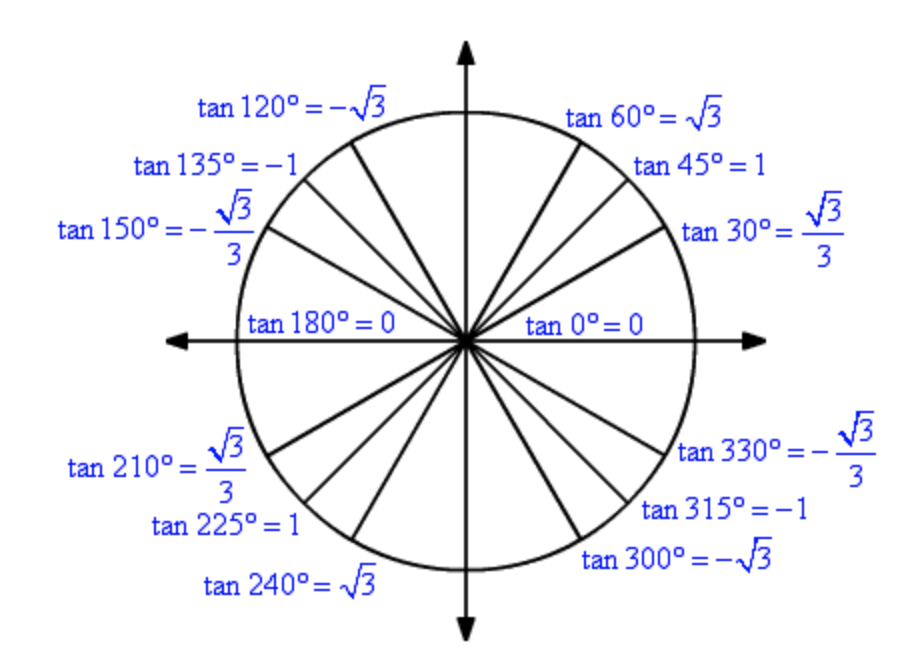
\includegraphics[width= 6cm]{images/tan3.png}
\end{center}
 \\
 \normalsize{ \cite{test1}\cite{varsitytutors}The tangent function is undefined when $x$ $=$ $\pi$ / 2 $+$ $n \pi$ (where, $n$ is integer) for which, $cos(x) = 0$. However, Tangent function does not have an amplitude. In addition, The graph intercept $x$-axis at $n\pi$ (where $n$ is integer) and in $y$-axis at $(0,0)$ point. The period of tangent function is $\pi$.
 }
 \\
 \subsection*{Range}\cite{test1}\cite{varsitytutors}
 \normalsize{ The range of $tan(x)$ is all real number $\mathbb{R}$, $(- \infty, + \infty)$. }
 
 \subsection*{Domain and Co-domain}\cite{test1}\cite{varsitytutors}
 \normalsize{The domain of tangent function is $x \in$ $\mathbb{R}$, $x$ $\neq$ $\pi$ / 2 $+$ $n \pi$ where, $n$ is an integer. The co-domain of $tan(x)$ is \((-\infty, +\infty\)).}

\pagebreak
\newpage
\addcontentsline{toc}{subsection}{b) Context of Use Model}
\section*{b)Context of Use Model}
\normalsize{Users can use the calculator to calculate the result of $sin()$, $cos()$ and $\frac{sin()}{cos()}$ which is $tan()$ of a degree. This degree shall be an integer or decimal, so the digits \textit{0-9} and the decimal point must be available by the user. The user can select the appropriate function they want to use, and they shall be able to press a button to have the answer computed. The calculator should return the result or an error message that indicates why it was unable to do so.}
\begin{center}
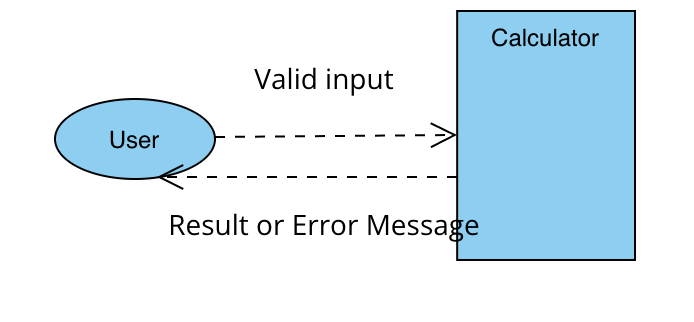
\includegraphics[width=15cm]{context_diagram}
\end{center}
\pagebreak
\newpage
\addcontentsline{toc}{section}{2) Problem 2}
\section*{2)Problem 2}
\subsection*{Assumption:} 
 For the given degree x, return the result of $tan(x)$. If the input value is invalid or cannot be calculated, return an error message.

\\
\subsection*{Requirements:} \\
\textbf{Functional Requirements:}\\
\newline
\begin{tabular}{ |c|c| } 
 \hline
 \textbf{Requirement Id} & FR1 \\ 
   \hline
 \textbf{Overview} & $x = 0^\circ $ + $n\pi$  \\
  \hline
  \textbf{Description} & 
\begin{tabular}[c]{@{}l@{}} For the given input $x = 0^\circ $ ,
the function \\may return 0 as output.
\end{tabular} \\
  \hline
\textbf{Priority} & High \\ 
  \hline
\textbf{Type} & Functional \\
  \hline
\textbf{Difficulty} & Easy \\
  \hline
\end{tabular}

\bigskip

\begin{tabular}{ |c|c|  } 
 \hline
 \textbf{Requirement Id} & FR2 \\ 
   \hline
 \textbf{Overview} &  x is Positive Degree  \\
  \hline
  \textbf{Description} & 
\begin{tabular}[c]{@{}l@{}} For the given input x = any Positive Degree  ,\\
the function may return corresponding\\ $tan(x)$ value as output.
\end{tabular} \\
  \hline
\textbf{Priority} & High \\ 
  \hline
\textbf{Type} & Functional \\
  \hline
\textbf{Difficulty} & Medium \\
  \hline
\end{tabular}\\
\bigskip
\newline
{\leftskip=0cm\relax
\begin{tabular}{ |c|c|  } 
 \hline
 \textbf{Requirement Id} & FR3 \\ 
   \hline
 \textbf{Overview} &  x is Negative  Degree  \\
  \hline
  \textbf{Description} & 
\begin{tabular}[c]{@{}l@{}} For the given input x = any Negative Degree  ,\\
the function may return corresponding\\ $tan(x)$ value as output.
\end{tabular} \\
  \hline
\textbf{Priority} & High \\ 
  \hline
\textbf{Type} & Functional \\
  \hline
\textbf{Difficulty} & Medium \\
  \hline
\end{tabular}\\
\bigskip
\newline
\begin{tabular}{ |c|c| } 
 \hline
 \textbf{Requirement Id} & FR4 \\ 
   \hline
 \textbf{Overview} & $x = 90^\circ$ + $n\pi$  \\
  \hline
  \textbf{Description} & 
\begin{tabular}[c]{@{}l@{}} For the given input x ,
the function \\may return "Invalid" as output.
\end{tabular} \\
  \hline
\textbf{Priority} & High \\ 
  \hline
\textbf{Type} & Functional \\
  \hline
\textbf{Difficulty} & Hard \\
  \hline
\end{tabular}\\
\pagebreak
\newpage
\textbf{Non-Functional Requirements:}\\
\newline
\begin{tabular}{ |c|c| } 
 \hline
 \textbf{Requirement Id} & NFR1 \\ 
   \hline
 \textbf{Overview} & Maintainability \\
  \hline
  \textbf{Description} & \begin{tabular}[c]{@{}l@{}} The ability to add features or fix bugs\\ after the project is finihed.
the function \\may return "Invalid" as output.
\end{tabular} \\
  \hline
\textbf{Priority} & High \\ 
  \hline
\textbf{Type} & NonFunctional \\
  \hline
\textbf{Difficulty} & Medium \\
  \hline
\end{tabular}\\
\bigskip
\newline
\begin{tabular}{ |c|c| } 
 \hline
 \textbf{Requirement Id} & NFR2 \\ 
   \hline
 \textbf{Overview} & Usability \\
  \hline
  \textbf{Description} & \begin{tabular}[c]{@{}l@{}} The ability that users can easily use its functions .
\end{tabular} \\
  \hline
\textbf{Priority} & High \\ 
  \hline
\textbf{Type} & NonFunctional \\
  \hline
\textbf{Difficulty} & Medium \\
  \hline
\end{tabular}
\bigskip
\newline
\begin{tabular}{ |c|c| } 
 \hline
 \textbf{Requirement Id} & NFR3 \\ 
   \hline
 \textbf{Overview} & Portability \\
  \hline
  \textbf{Description} & \begin{tabular}[c]{@{}l@{}} The ability that the project can \\easily suit in users' system environment .
\end{tabular} \\
  \hline
\textbf{Priority} & High \\ 
  \hline
\textbf{Type} & NonFunctional \\
  \hline
\textbf{Difficulty} & High \\
  \hline
\end{tabular}

\pagebreak
\newpage
\addcontentsline{toc}{section}{3) Problem 3}
\section*{3)Problem 3}
\addcontentsline{toc}{subsection}{a) Algorithm Selection}
\subsection*{a)Algorithm Selection}
For this part, I will introduce two algorithms for implementing $tan(x)$ function. \textbf{Polynomial approximation and Maclaurin series.}\\
\newline
\textbf{Algorithm1 : Polynomial approximation} }\\
\newline
\cite{poly}Polynomial approximation is an approximation of a curve with a polynomial. When we solve mathematical questions, we don't actually know how to calculate certain functions, such as the $sin()$ function. Therefore, to solve this kind of problems, mathematicians develop very good approximations to these functions - related functions which are very close to the function of interest, but much easier to calculate.\\
\newline
\begin{tabular}{ |c|c|}
\hline
\textbf{Advantages} & \textbf{Disadvantages}\\ \hline 
Easy to calculate
 & \makecell{The approximation is only precise for small x, so some steps are \\needed when we calculate $tan(x)$} \\
\hline

\end{tabular} \\ \\

\newline
\textbf{Algorithm2 : Maclaurin series}\\
\newline
\cite{macl}A Maclaurin series is a Taylor series expansion of a function about 0,\\
 \begin{center}
$f(x) = f(0)+f'(0)x + \frac{f''(0)}{2!}x^2 + \frac{f^{(3)}(0)}{3!}x^3 + ...  + \frac{f^{(n)}(0)}{n!}x^n$\\
\end{center}
\newline
The $tan(x)$ function's approximation is derived by the Maclaurin Series's explicit forms of $sin(x)$ and $cos(x)$.
\begin{equation} 
sin(x) = x-x^3/3!+x^5/5!-x^7/7!+.....
\end{equation}
\begin{equation} 
cos(x) = 1-x^2/2!+x^4/4!-x^6/6!+.....
\end{equation}\\
Then, we can use $\tan(x)$ = $\frac{sin(x)}{cos(x)}$ to calculate.\\
\newline
\begin{tabular}{ |c|c|}
\hline
\textbf{Advantages} & \textbf{Disadvantages}\\ \hline 
\makecell{The formula  $\tan(x)$ = $\frac{sin(x)}{cos(x)}$ \\is easy to understand.}
 & \makecell{Successive terms get very complex and hard to derive.} \\
\hline

\end{tabular} \\ \\
\pagebreak
\newpage
\addcontentsline{toc}{subsection}{b) Mind Map for Pseudocode Format}
\subsection*{b)Mind Map For Pseudocode}
In this part, I will use a mind map to decide a pseudocode format.\\

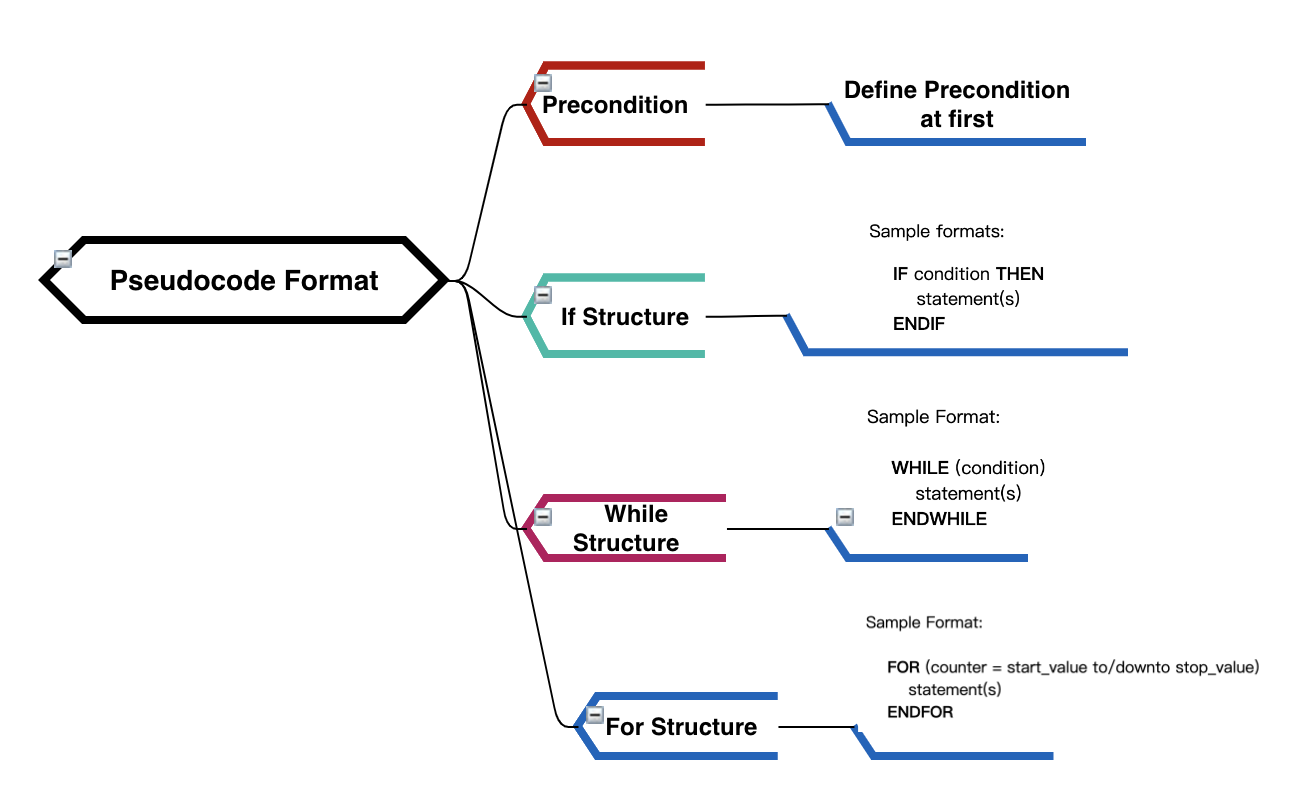
\includegraphics[width= 14cm]{images/mindmap.png}
 \\
 
\addcontentsline{toc}{subsection}{c) Pseudocode for each Algorithm}
\subsection*{c) Pseudocode for each Algorithm}
In this part, I will write pseudocode for each algorithm.\\
\begin{algorithm}
\caption{\cite{pseupoly}Polynomial approximation} \label{alg:cap}
\begin{algorithmic}
\Require $x \notin [0^\circ,180^\circ]$ 
\Function{periodicity}{x}
\If{$x>180^\circ$}
\While{$x>180^\circ$}
\State $x = x-180^\circ$\Comment{reduce x to the range $[0^\circ,180^\circ]$}
\EndWhile 
\Else
       \While{$x<0^\circ$}
\State $x = x+180^\circ$\Comment{add x to the range $[0^\circ,180^\circ]$}
\EndWhile 
\EndIf\\   
\Return{$x$}\Comment{get valid x}
\EndFunction
\end{algorithmic}
\end{algorithm}
\begin{algorithm}
\begin{algorithmic}
\Require $x \notin [0^\circ,90^\circ]$ 
\Function{symmetry}{x}
\State $tan(x)$ = -$tan(180^\circ-x)$\Comment{use the symmetry of $tan()$ }\\
\Return{$tan(x)$}\Comment{Return result}
\EndFunction\\
\newline
\Require $x \notin [0^\circ,45^\circ]$ 
\Function{cofunction}{x}
\State $tan(x)$ = -$\frac{1}{tan(90^\circ-x)}$\Comment{use the reciprocal of $tan()$ }\\
\Return{$tan(x)$}\Comment{Return result}
\EndFunction\\
\newline
\Require $x \notin [0^\circ,22.5^\circ]$ 
\Function{ trigonometric\_identity}{x}
\State $tan(x)$ = -$\frac{2tan(\frac{x}{2})}{1-tan^2(\frac{x}{2})}$\Comment{use the trig identity of $tan()$ }\\
\Return{$tan(x)$}\Comment{Return result}
\EndFunction\\
\newline
\Require $x \in [0^\circ,22.5^\circ]$ 
\Function{ polynomial}{x}
\State x = $x * \frac{\pi}{180^\circ}$\Comment{convert x to radians }
\State $tan(x)$ = $x+\frac{x^3}{3} + \frac{2x^5}{15} +\frac{17x^7}{315}$\Comment{use the trig identity of $tan()$ }\\
\Return{$tan(x)$}\Comment{Return result}
\EndFunction\\
\end{algorithmic}
\end{algorithm}
\begin{algorithm}
\caption{Maclaurin Series} \label{alg:cap}
\begin{algorithmic}
\Require x in degrees
\Function{getrad}{x}
\State $val = x * \frac{\pi}{180^\circ}$\Comment{Calculate x in radians}\\
\Return{$val$}\Comment{return x in radians}
\EndFunction
\newline
\Require $n\neq 0$ and $length = 0$ 
\Function{checkdigits}{n}
\While{$n\leqq1$}
\State $length += 1$\Comment{Calculate length}
\State $n *= 10$
\EndWhile\\
\Return{$length$}\Comment{return length}
\EndFunction
\end{algorithmic}
\end{algorithm}

\begin{algorithm}
\begin{algorithmic}
\Require $getrad(x)\neq NULL$ AND $n \neq 0$ AND x in radians AND $k = 1$ AND $m = 0$
\Function{CalculateSin}{getrad(x)}
\State $sinres = \frac{x}{k!}$
\While{$checkdigits(sinres)\neq n$}
\State $k = k+2$
\If{$m \% 2 ==0$}
\State $sinres -= \frac{x^k}{k!}$ 
\Else
\State $sinres += \frac{x^k}{k!}$ 
\EndIf
\State $m+=1$
\EndWhile\\
\Return{$sinres$}\Comment{get value of sin(x)}
\EndFunction\\
\newline
\Require $getrad(x)\neq NULL$ AND $n \neq 0$ AND x in radians AND $k = 2$ AND $m = 0$
\Function{CalculateCos}{getrad(x)}
\State $cosres = 1$
\While{$checkdigits(cosres)\neq n$}
\State $k = k+2$
\If{$m \% 2 ==0$}
\State $sinres -= \frac{x^k}{k!}$ 
\Else
\State $sinres += \frac{x^k}{k!}$ 
\EndIf
\State $m+=1$
\EndWhile\\
\Return{$cosres$}\Comment{get value of cos(x)}
\EndFunction\\

\Require $getrad(x)\neq NULL$ AND $ calculatecos(x)\neq NULL$ AND $calculatesin(x)\neq NULL$
\Function{Calculatetan}{calculatecos(x),calculatesin(x)}
\State SinVal = calculatesin(x)
\State CosVal = calculatecos(x)\\
\Return{$\frac{SinVal}{CosVal}$}\Comment{calculation for tan(x)}
\EndFunction
\State $result \gets $\Call{$tan(x)$}{}
\end{algorithmic}
\end{algorithm}
\pagebreak
\newpage
\addcontentsline{toc}{section}{4) Problem 4}
\section*{4)Problem 4}
\subsection*{a)Debugger}\\
\textbf{Description:}\\
\newline
The debugger I used is the Intellij IDEA built-in debugger. When I click the debug button, it will enter the debug mode. And in the debug mode, it will stop at the break point I set, and can go step by step. In addition to this, I can see the value of variables in each step.\\
\newline
\begin{tabular}{ |c|c|}
\hline
\textbf{Advantages} & \textbf{Disadvantages}\\ \hline No need to install,easy to use
 & \makecell{It may not support multi-threading program} \\
\hline
 Can see the value of variables in each step
 &  \\
 \hline
  It provide break point which can stop anywhere
 &  \\
 \hline
\end{tabular} \\ \\
\bigskip
\textbf{Example:}\\
1. Enter a valid input($195^\circ$), then press Tan button and "=" button\\
\newline
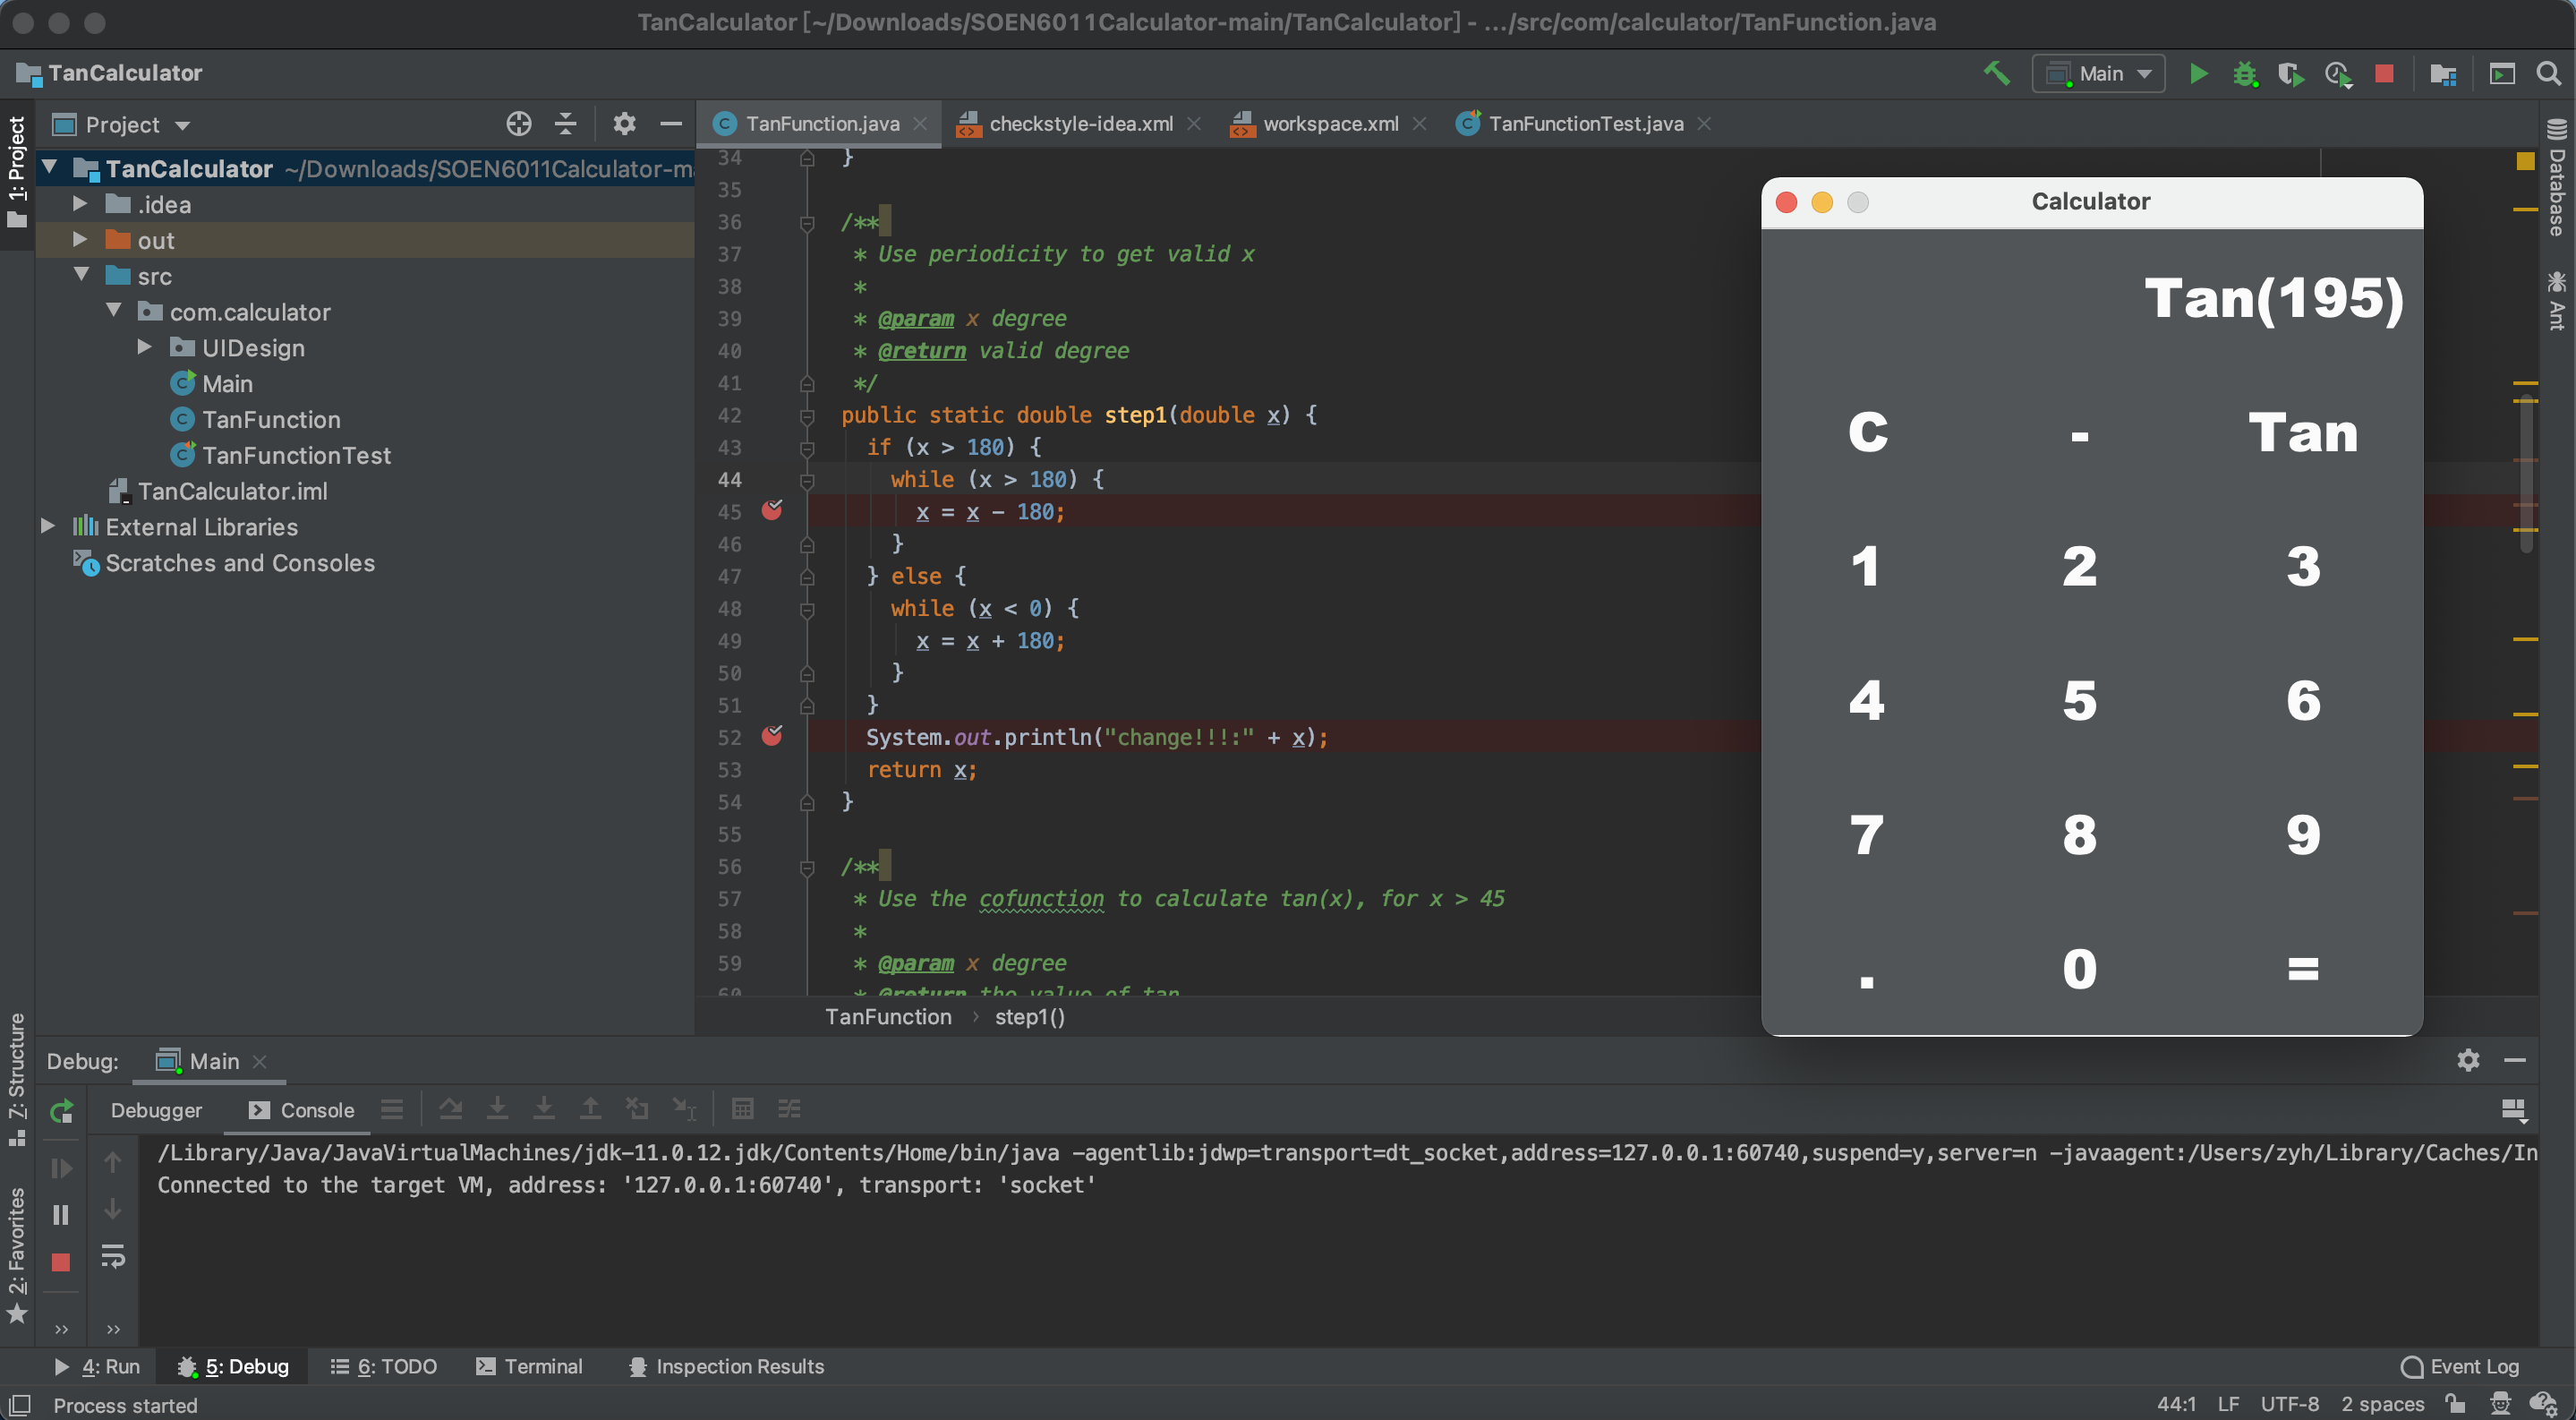
\includegraphics[width=15cm]{step1}\\
\newline
2. Go to calculateTan function and classify the degree.\\
\newline
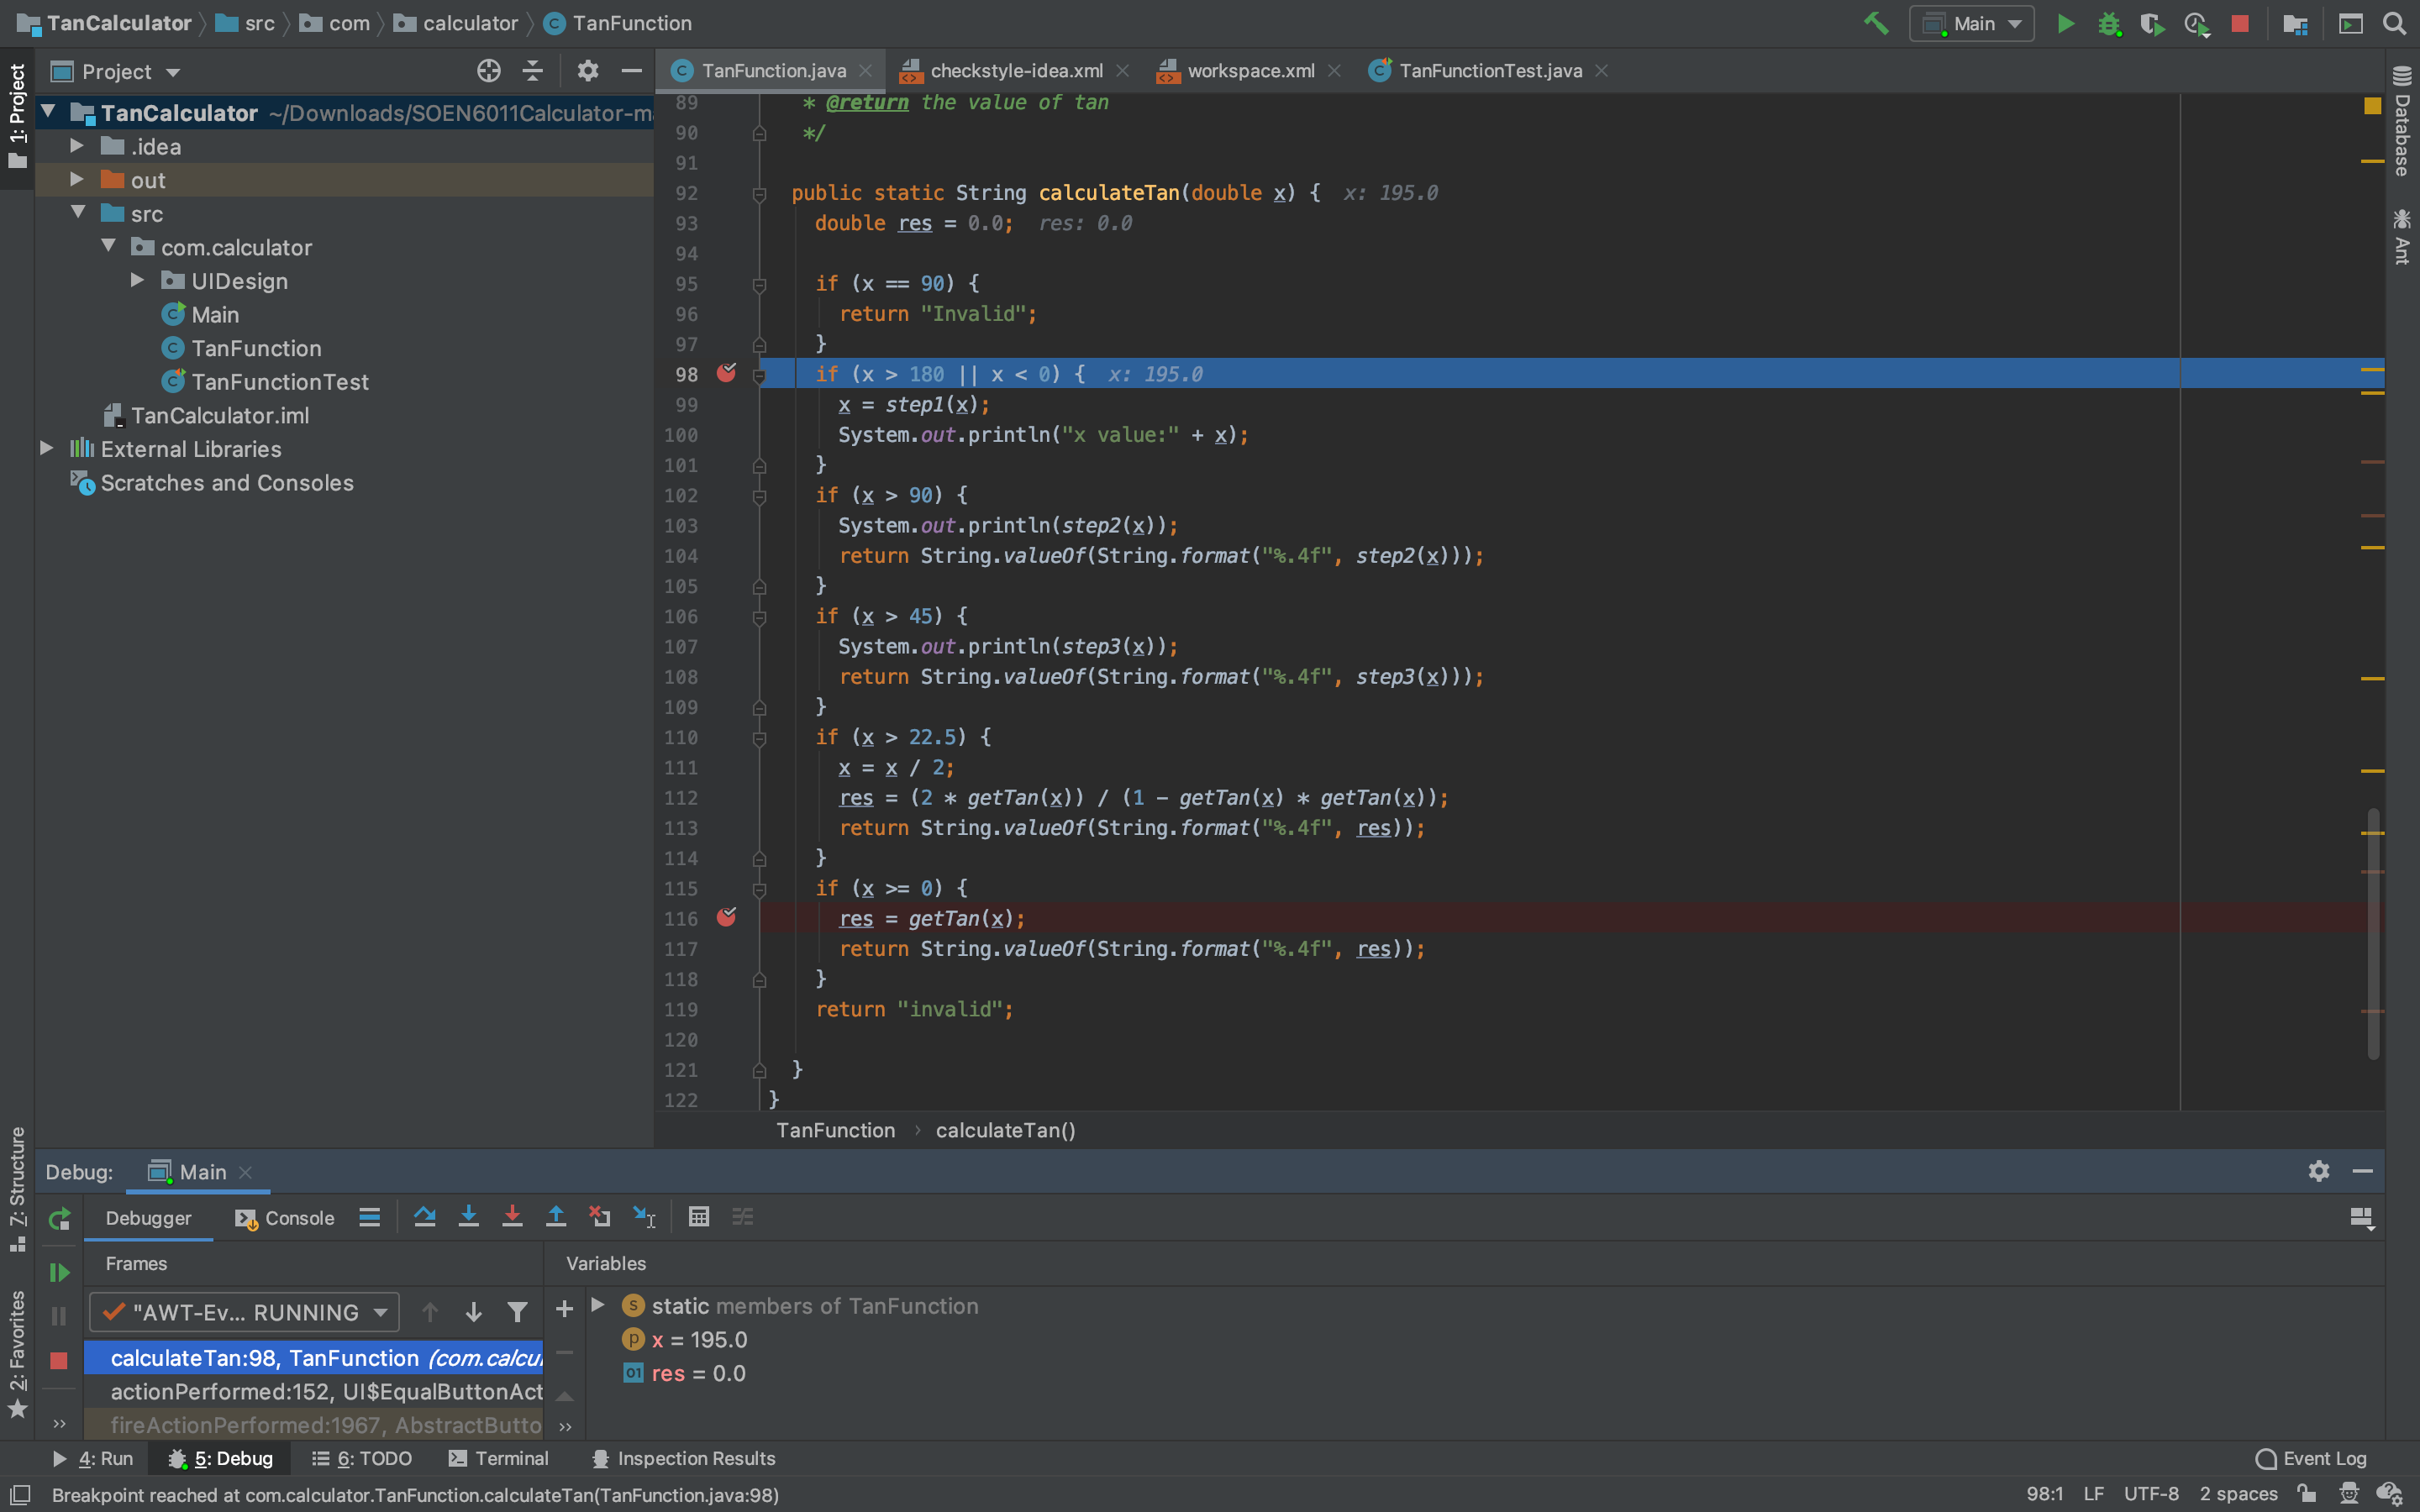
\includegraphics[width=15cm]{step2}\\
\newline
3. Go to step1 function and reduce it to the valid range.(We can see it decrease to $15^\circ $)\\
\newline
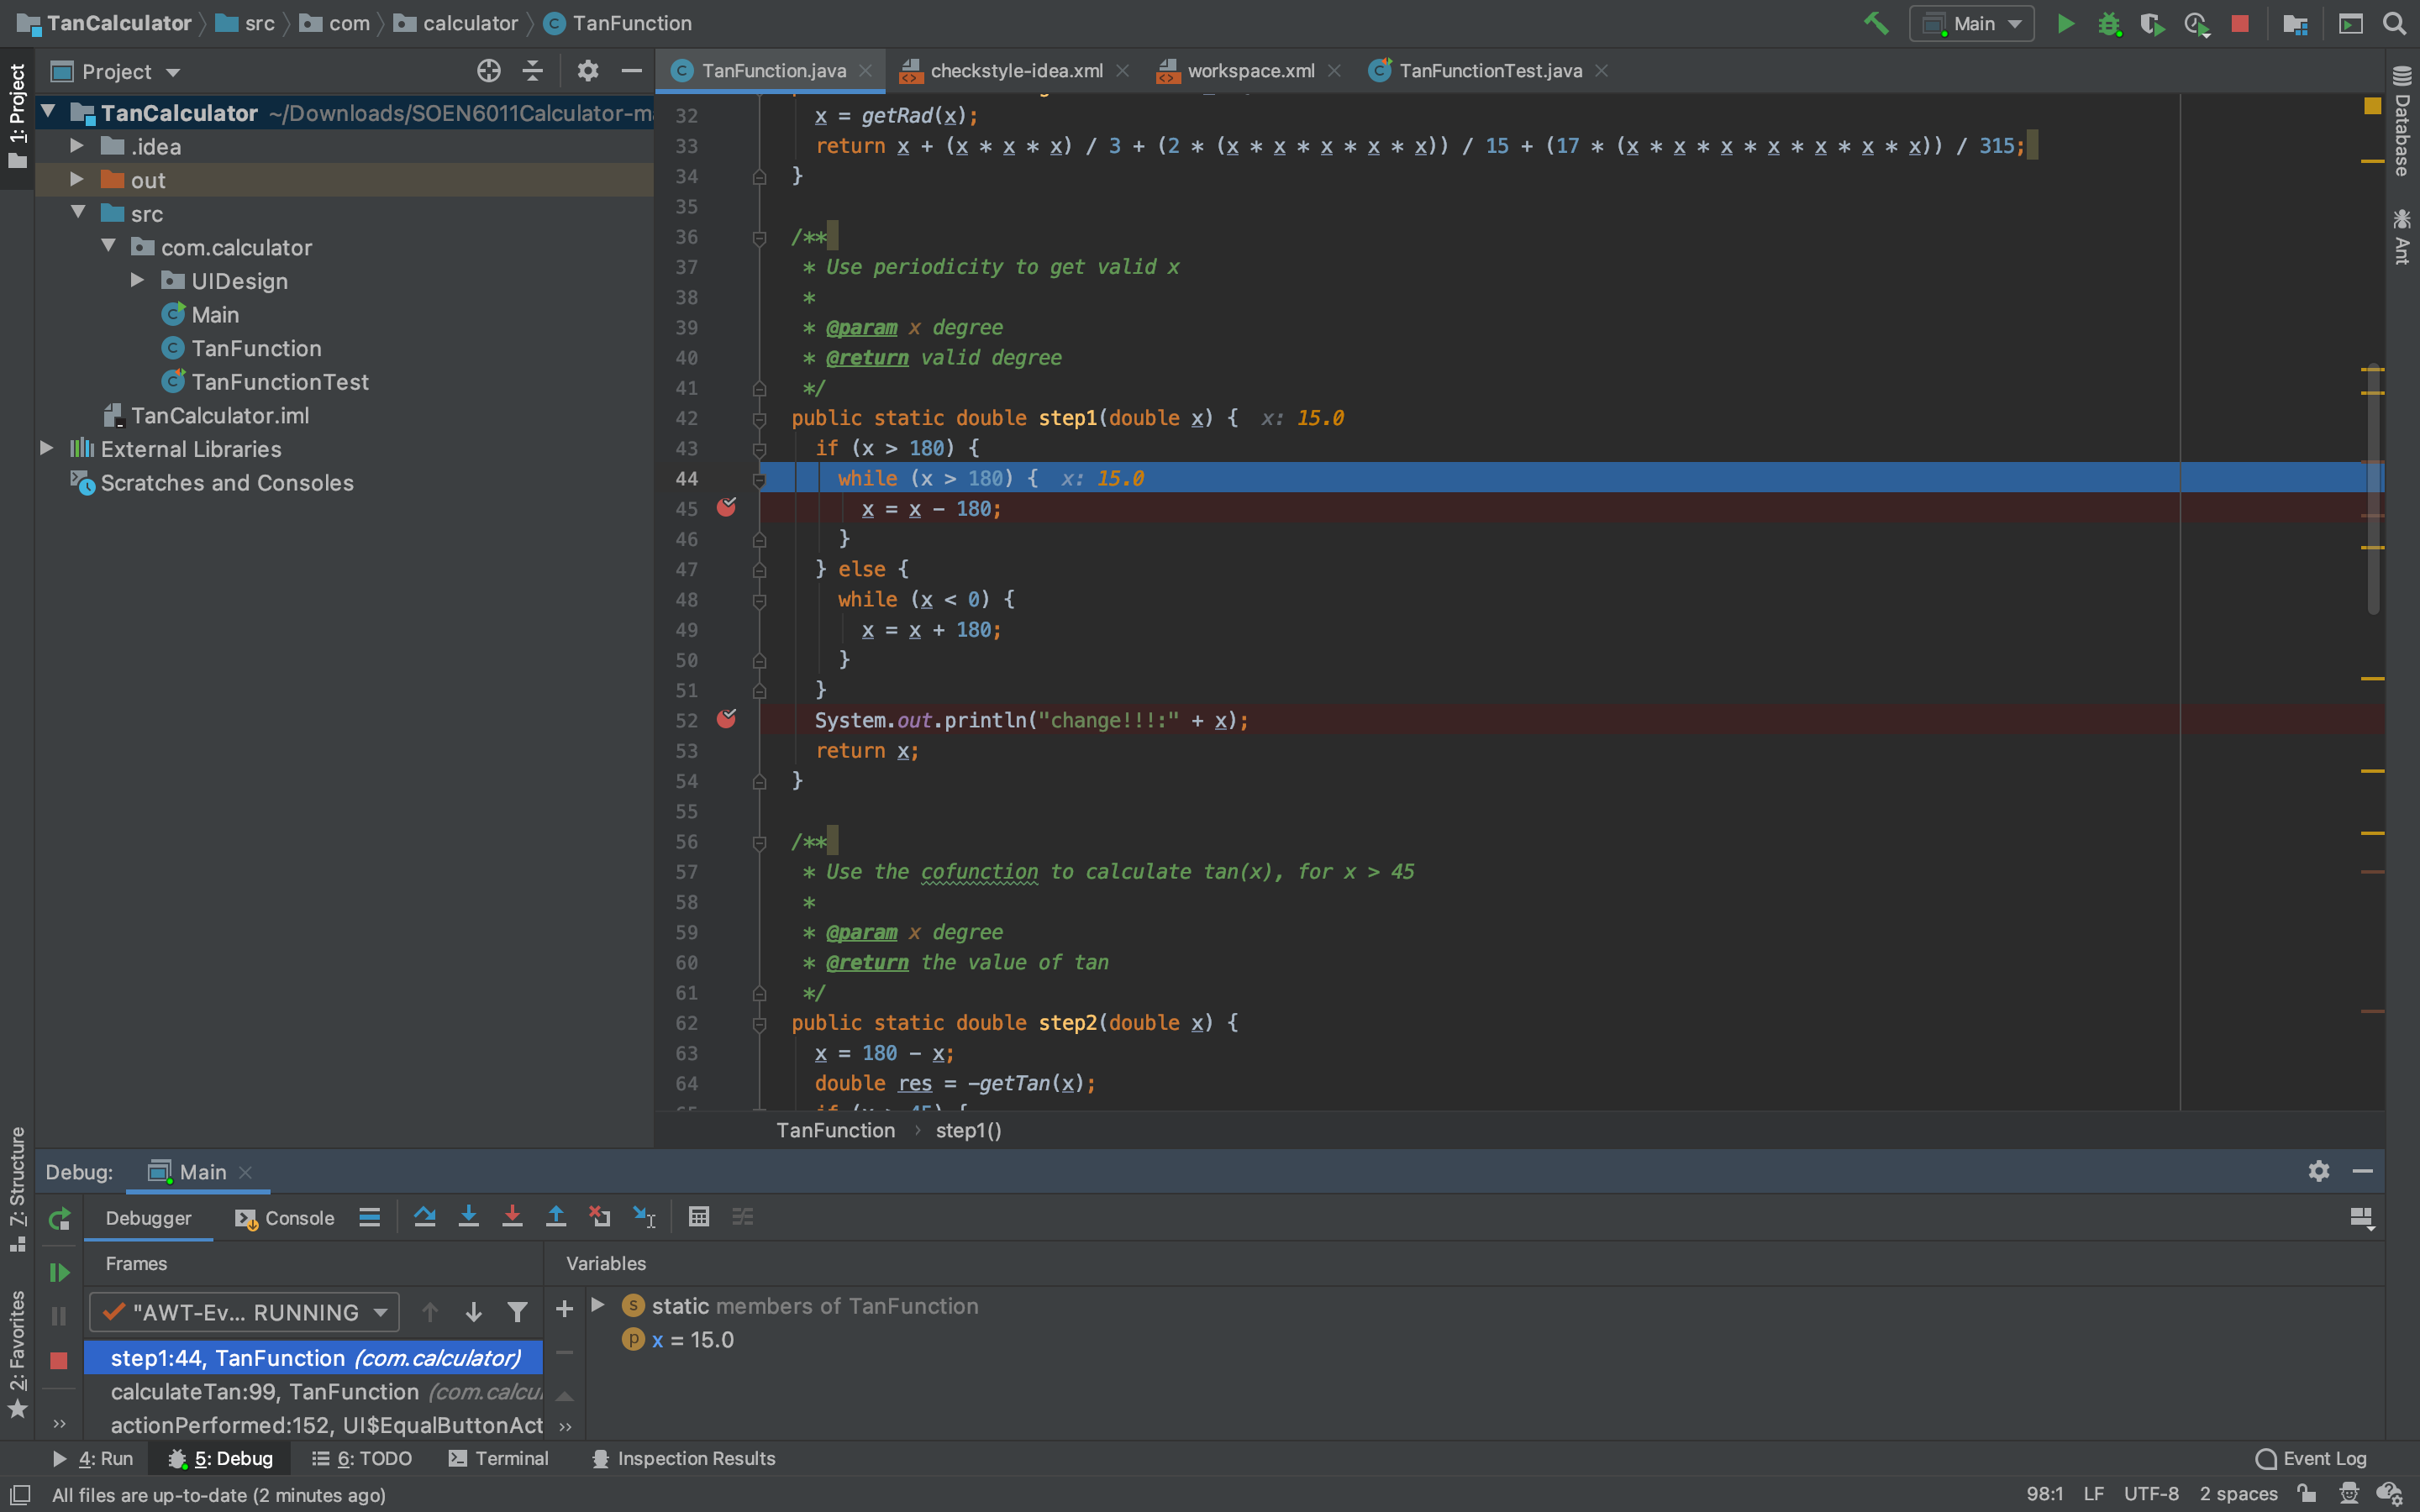
\includegraphics[width=15cm]{step3}\\
\pagebreak
\newpage
4. Return to calculateTan function and continue judge the degree.\\
\newline
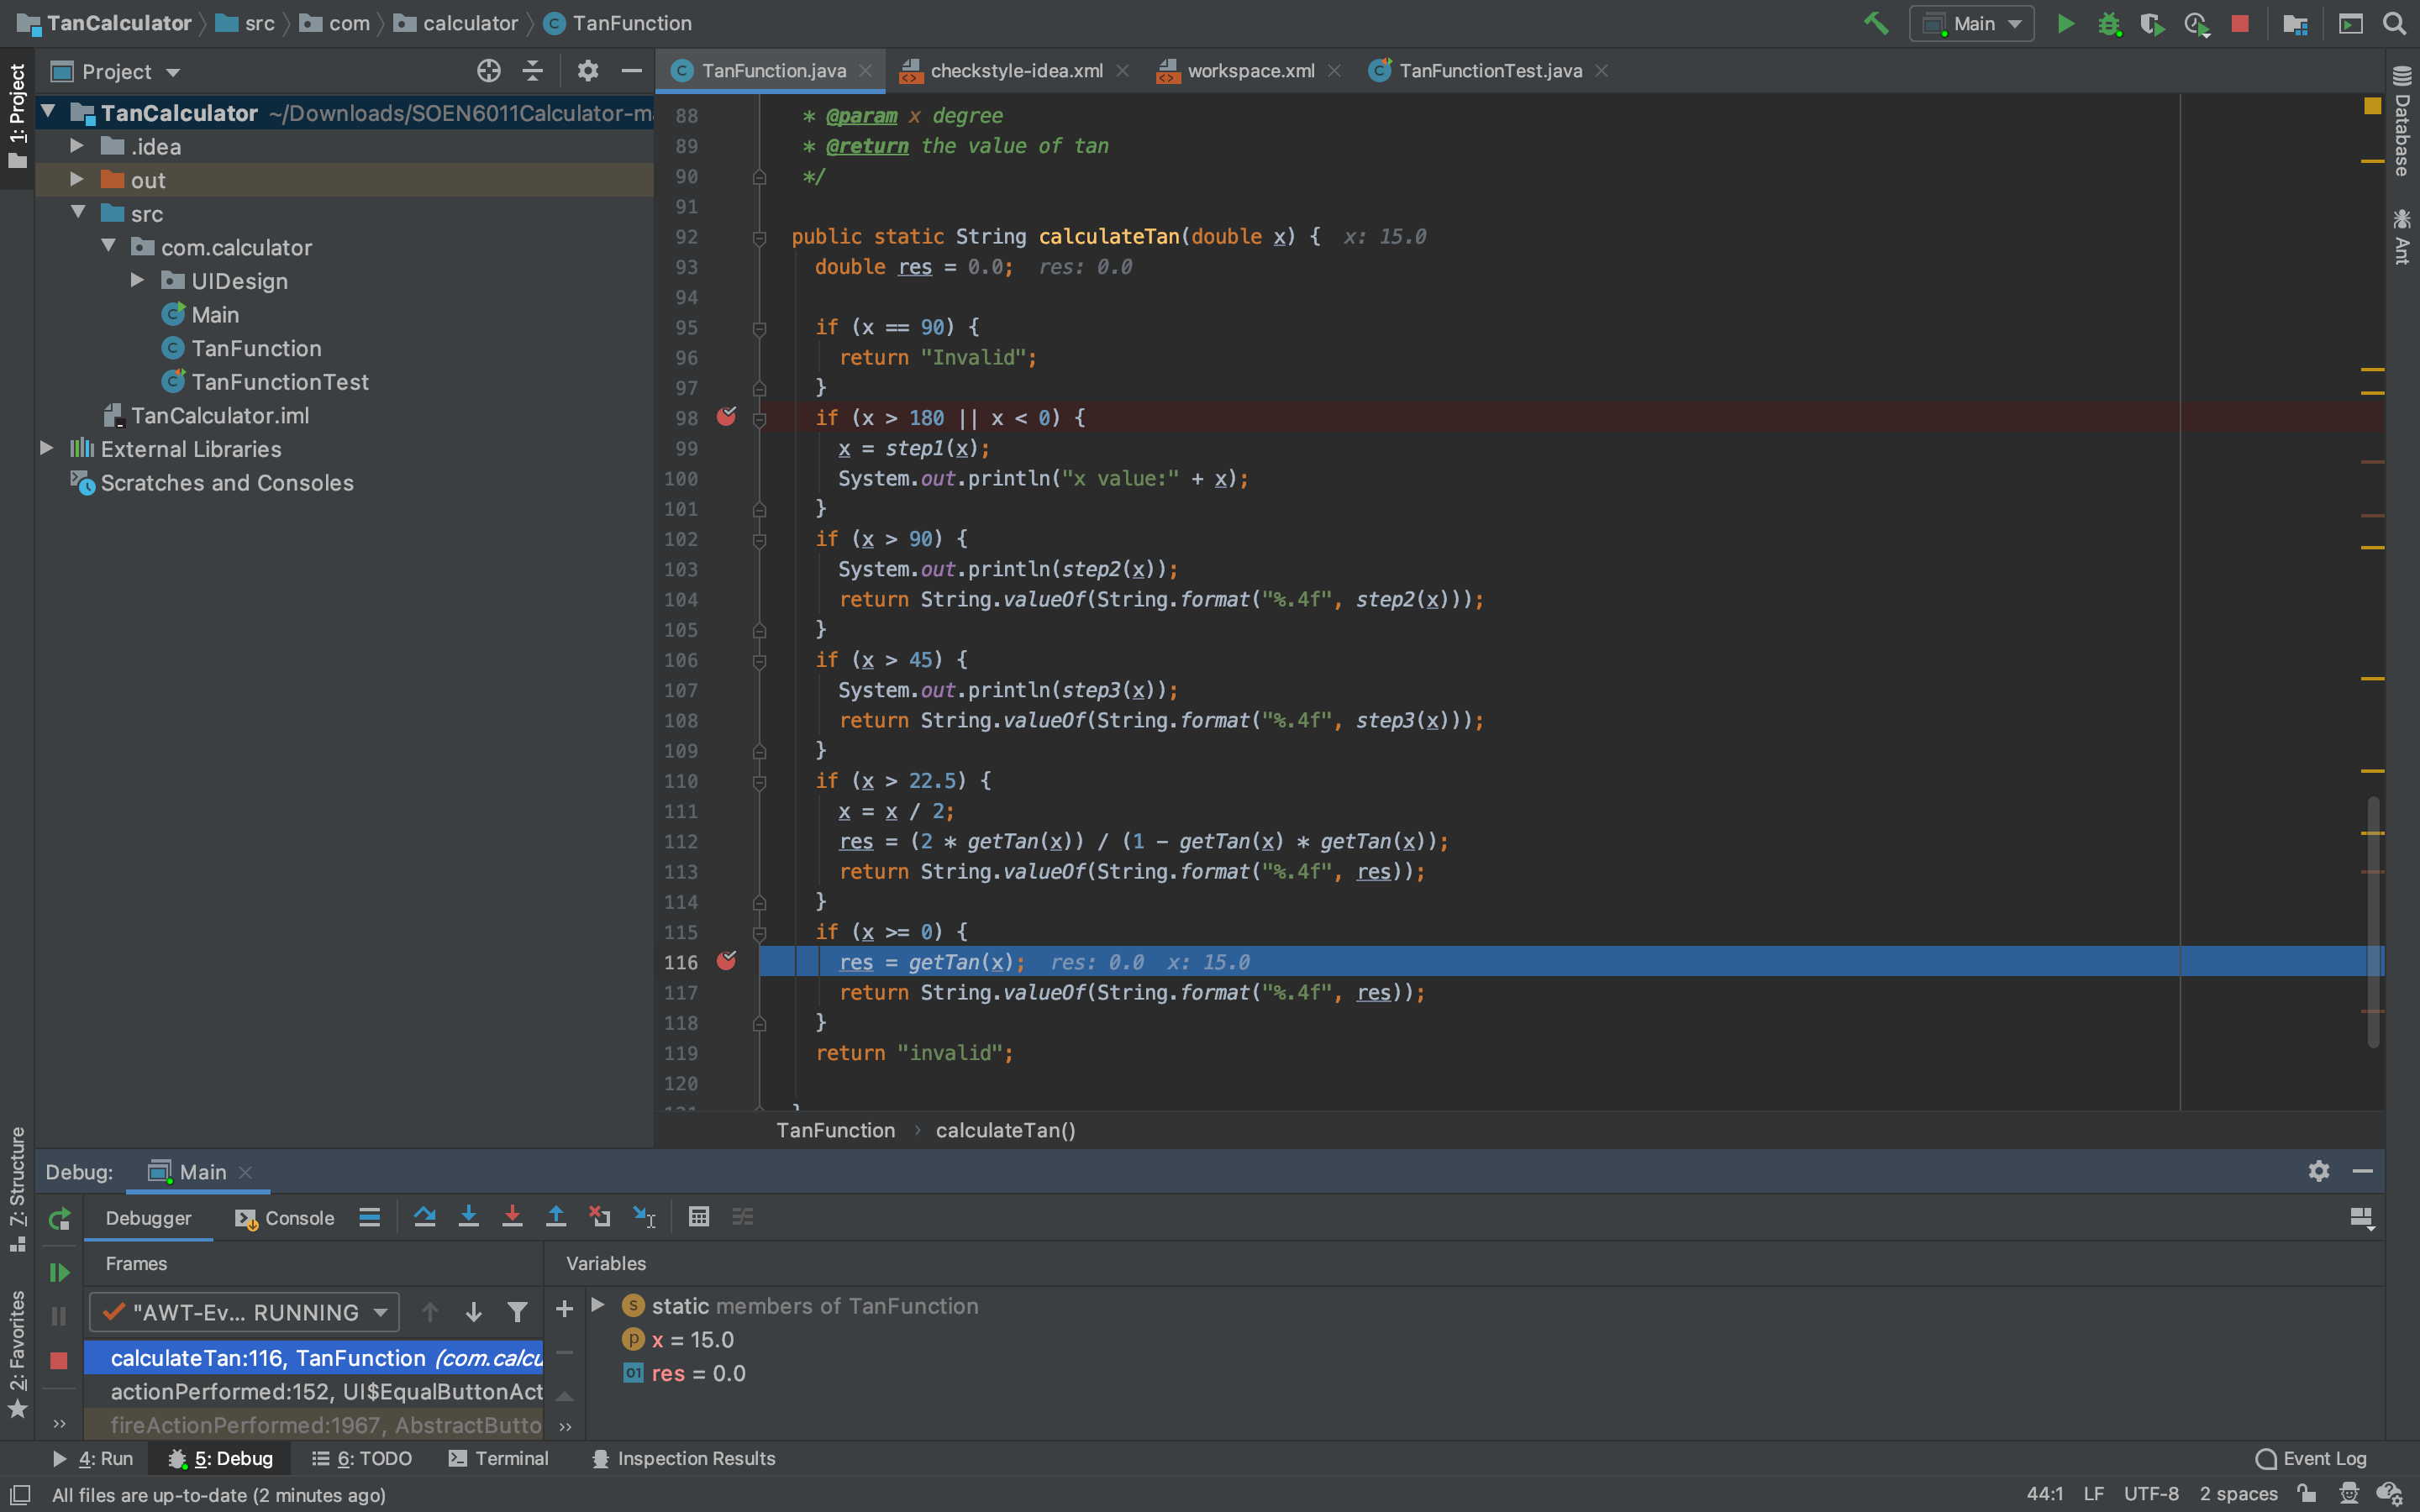
\includegraphics[width=15cm]{step4}\\
\newline
5. Go to getTan function to calculate the result.\\
\newline
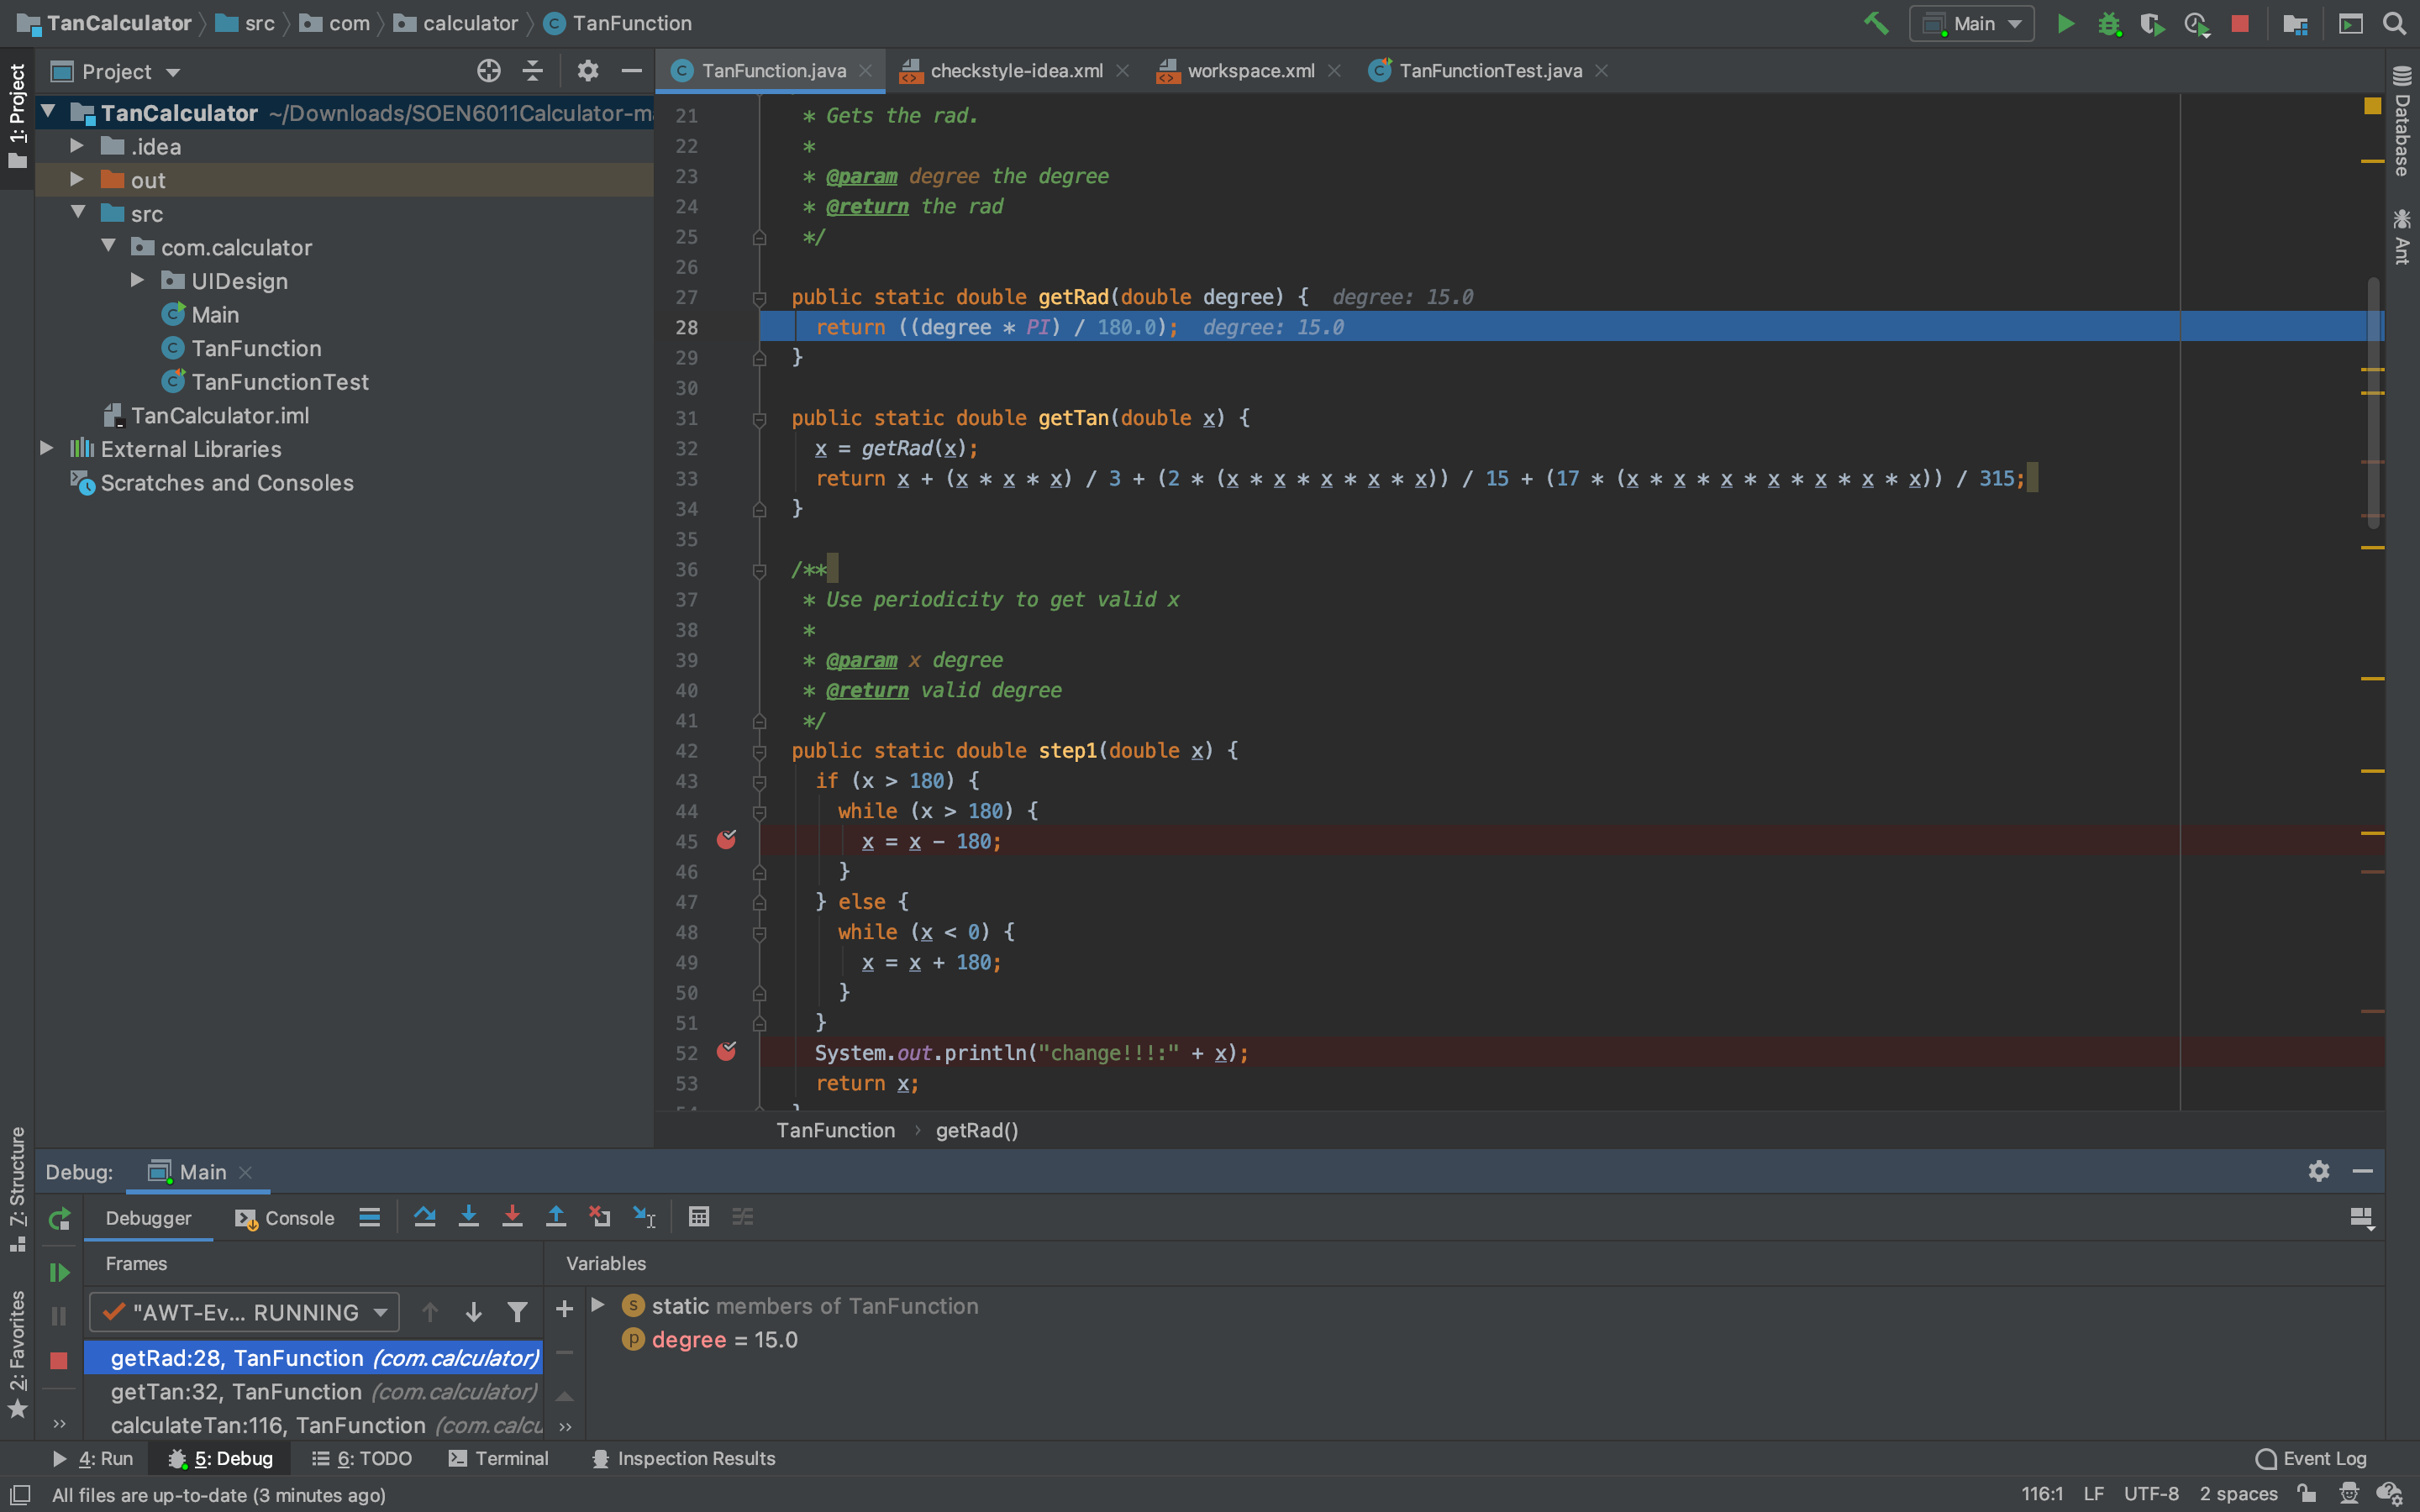
\includegraphics[width=15cm]{step5}\\
\pagebreak
\newpage
6.Get the result and return to UI function and display it on the interface.\\
\newline
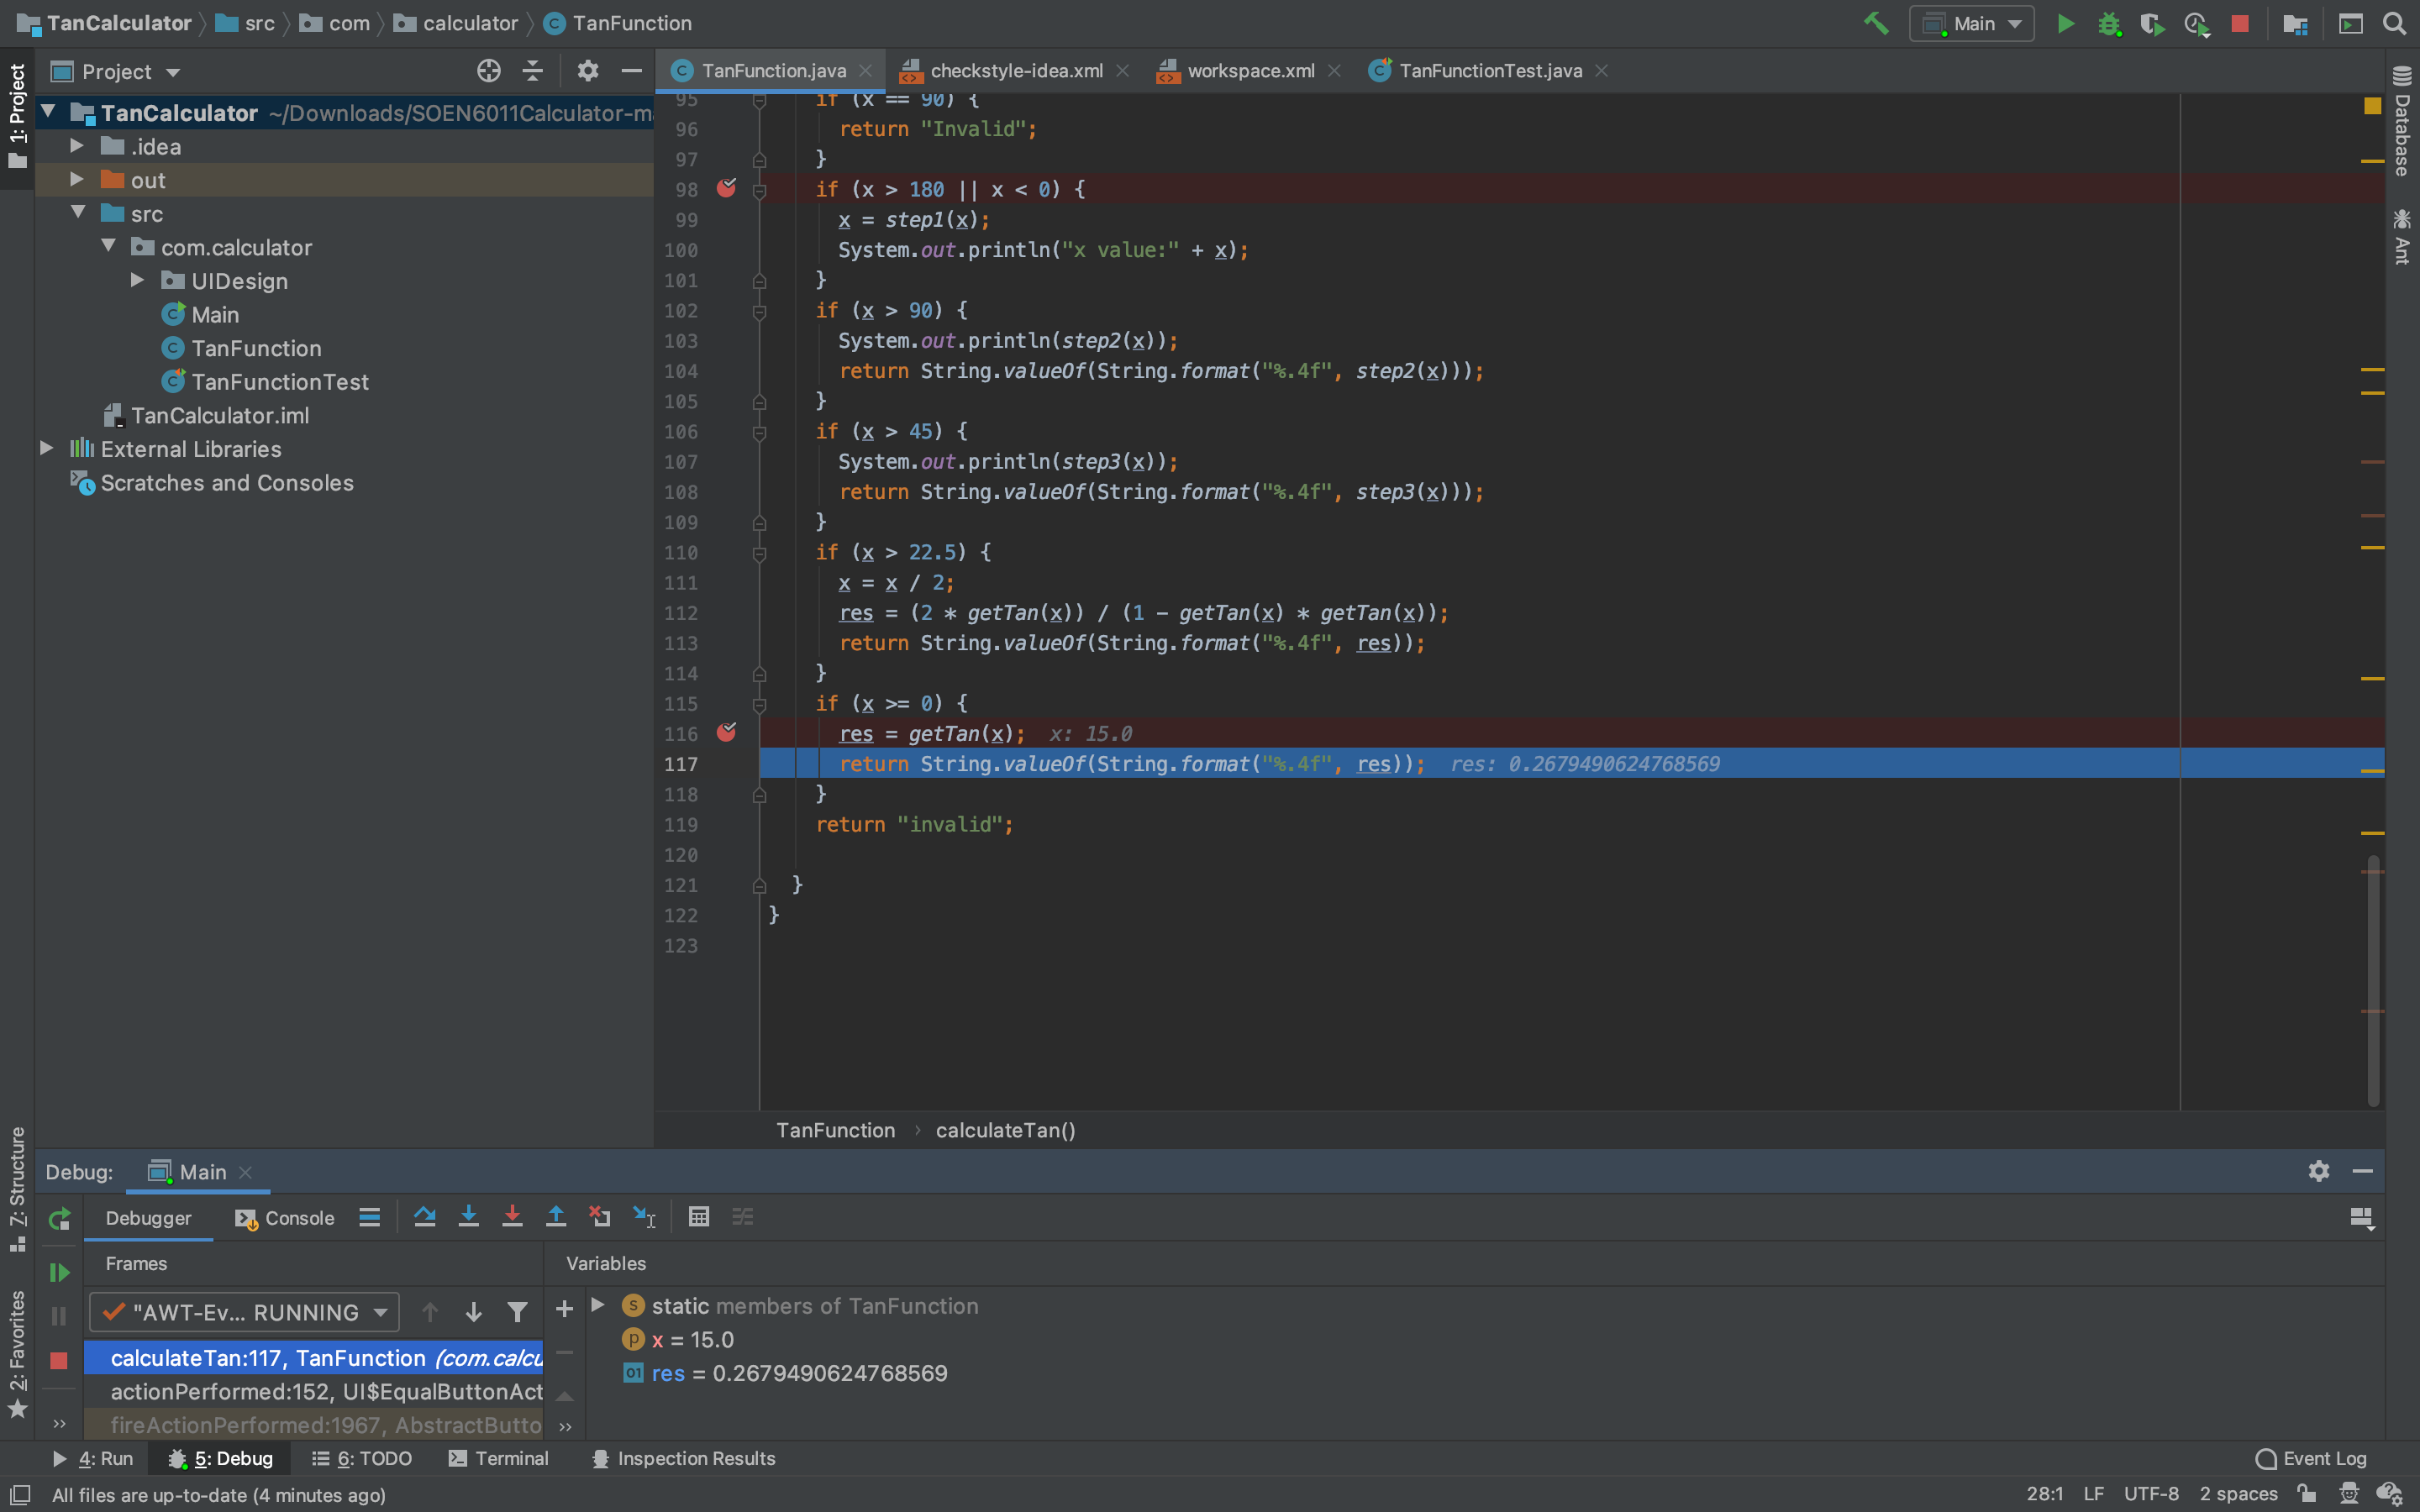
\includegraphics[width=15cm]{step6}\\
\newline
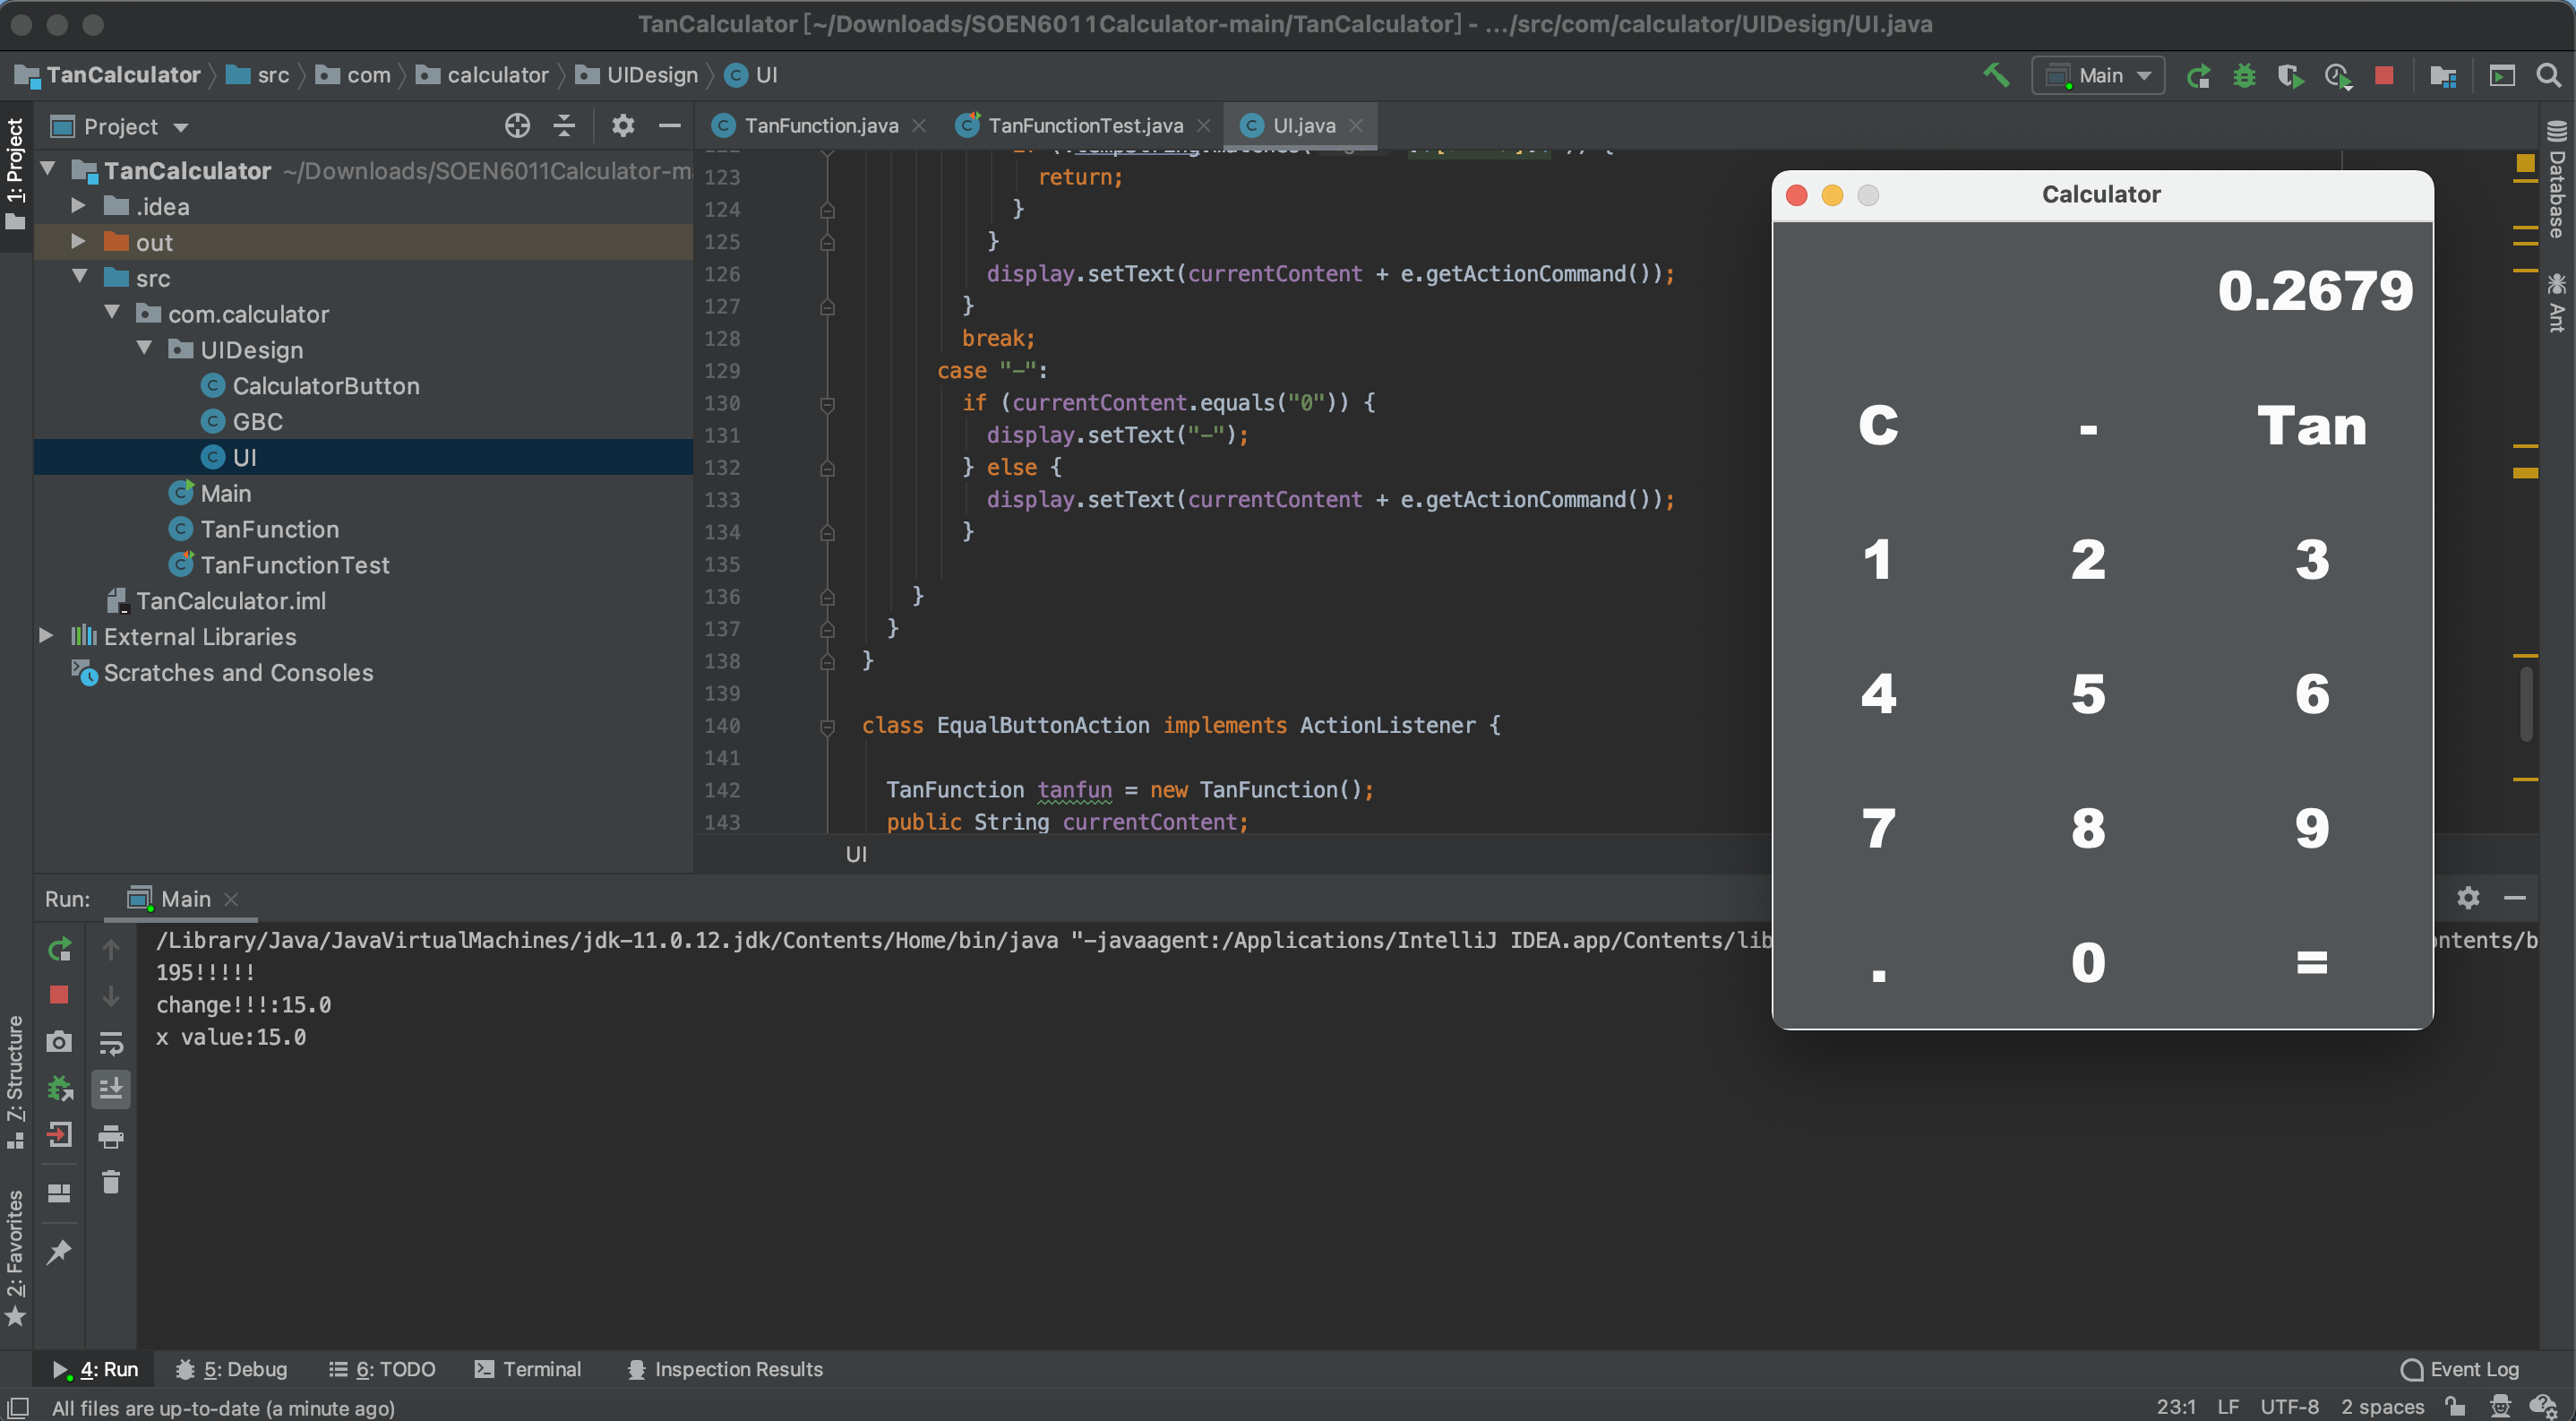
\includegraphics[width=15cm]{step7}\\
\pagebreak
\newpage

\subsection*{b)Error handling and Error Messaging}\\
If there is an invalid input, the system will catch an exception and return an error message. After receive an error message, users can reenter the valid input and get the result they want.\\
\newline
\textbf{Example:}\\
\newline
1.User click "Tan" button first then click number\\
\newline
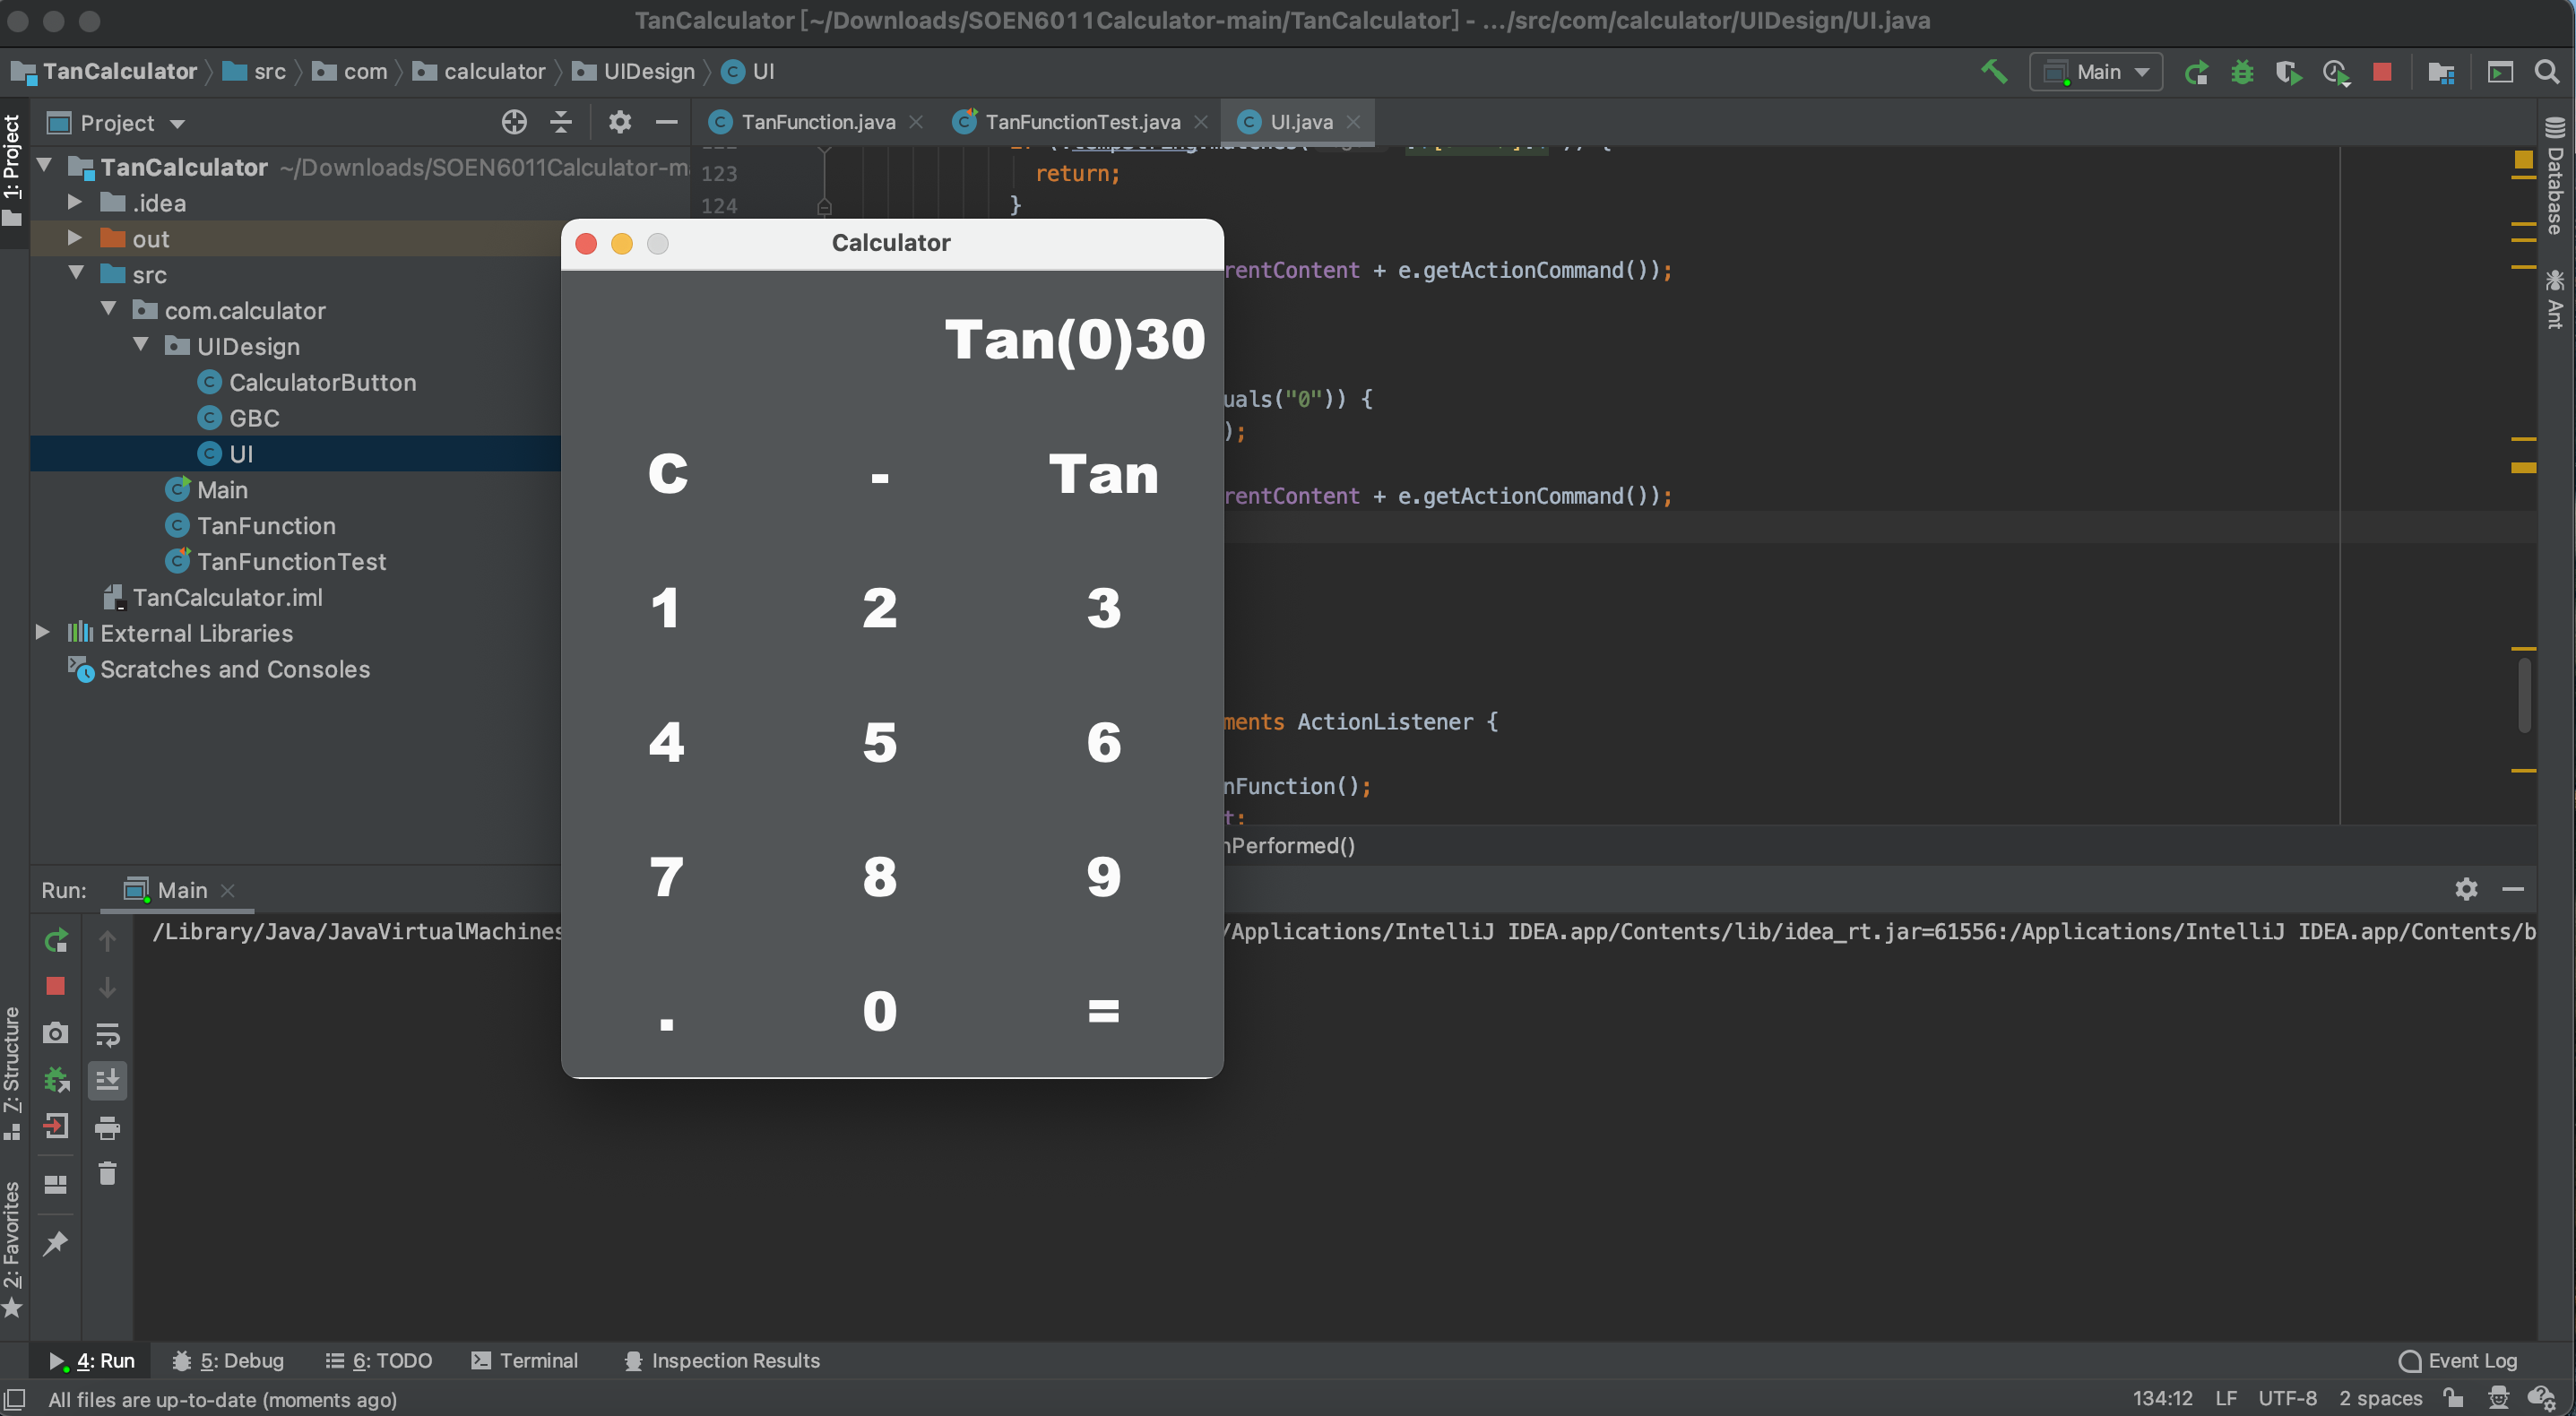
\includegraphics[width=13cm,height = 7cm]{err1}\\
\newline
2. After click "=" button, return an error message. And use can use "C" button to clear the text and reenter the number according to the error message.\\
\newline
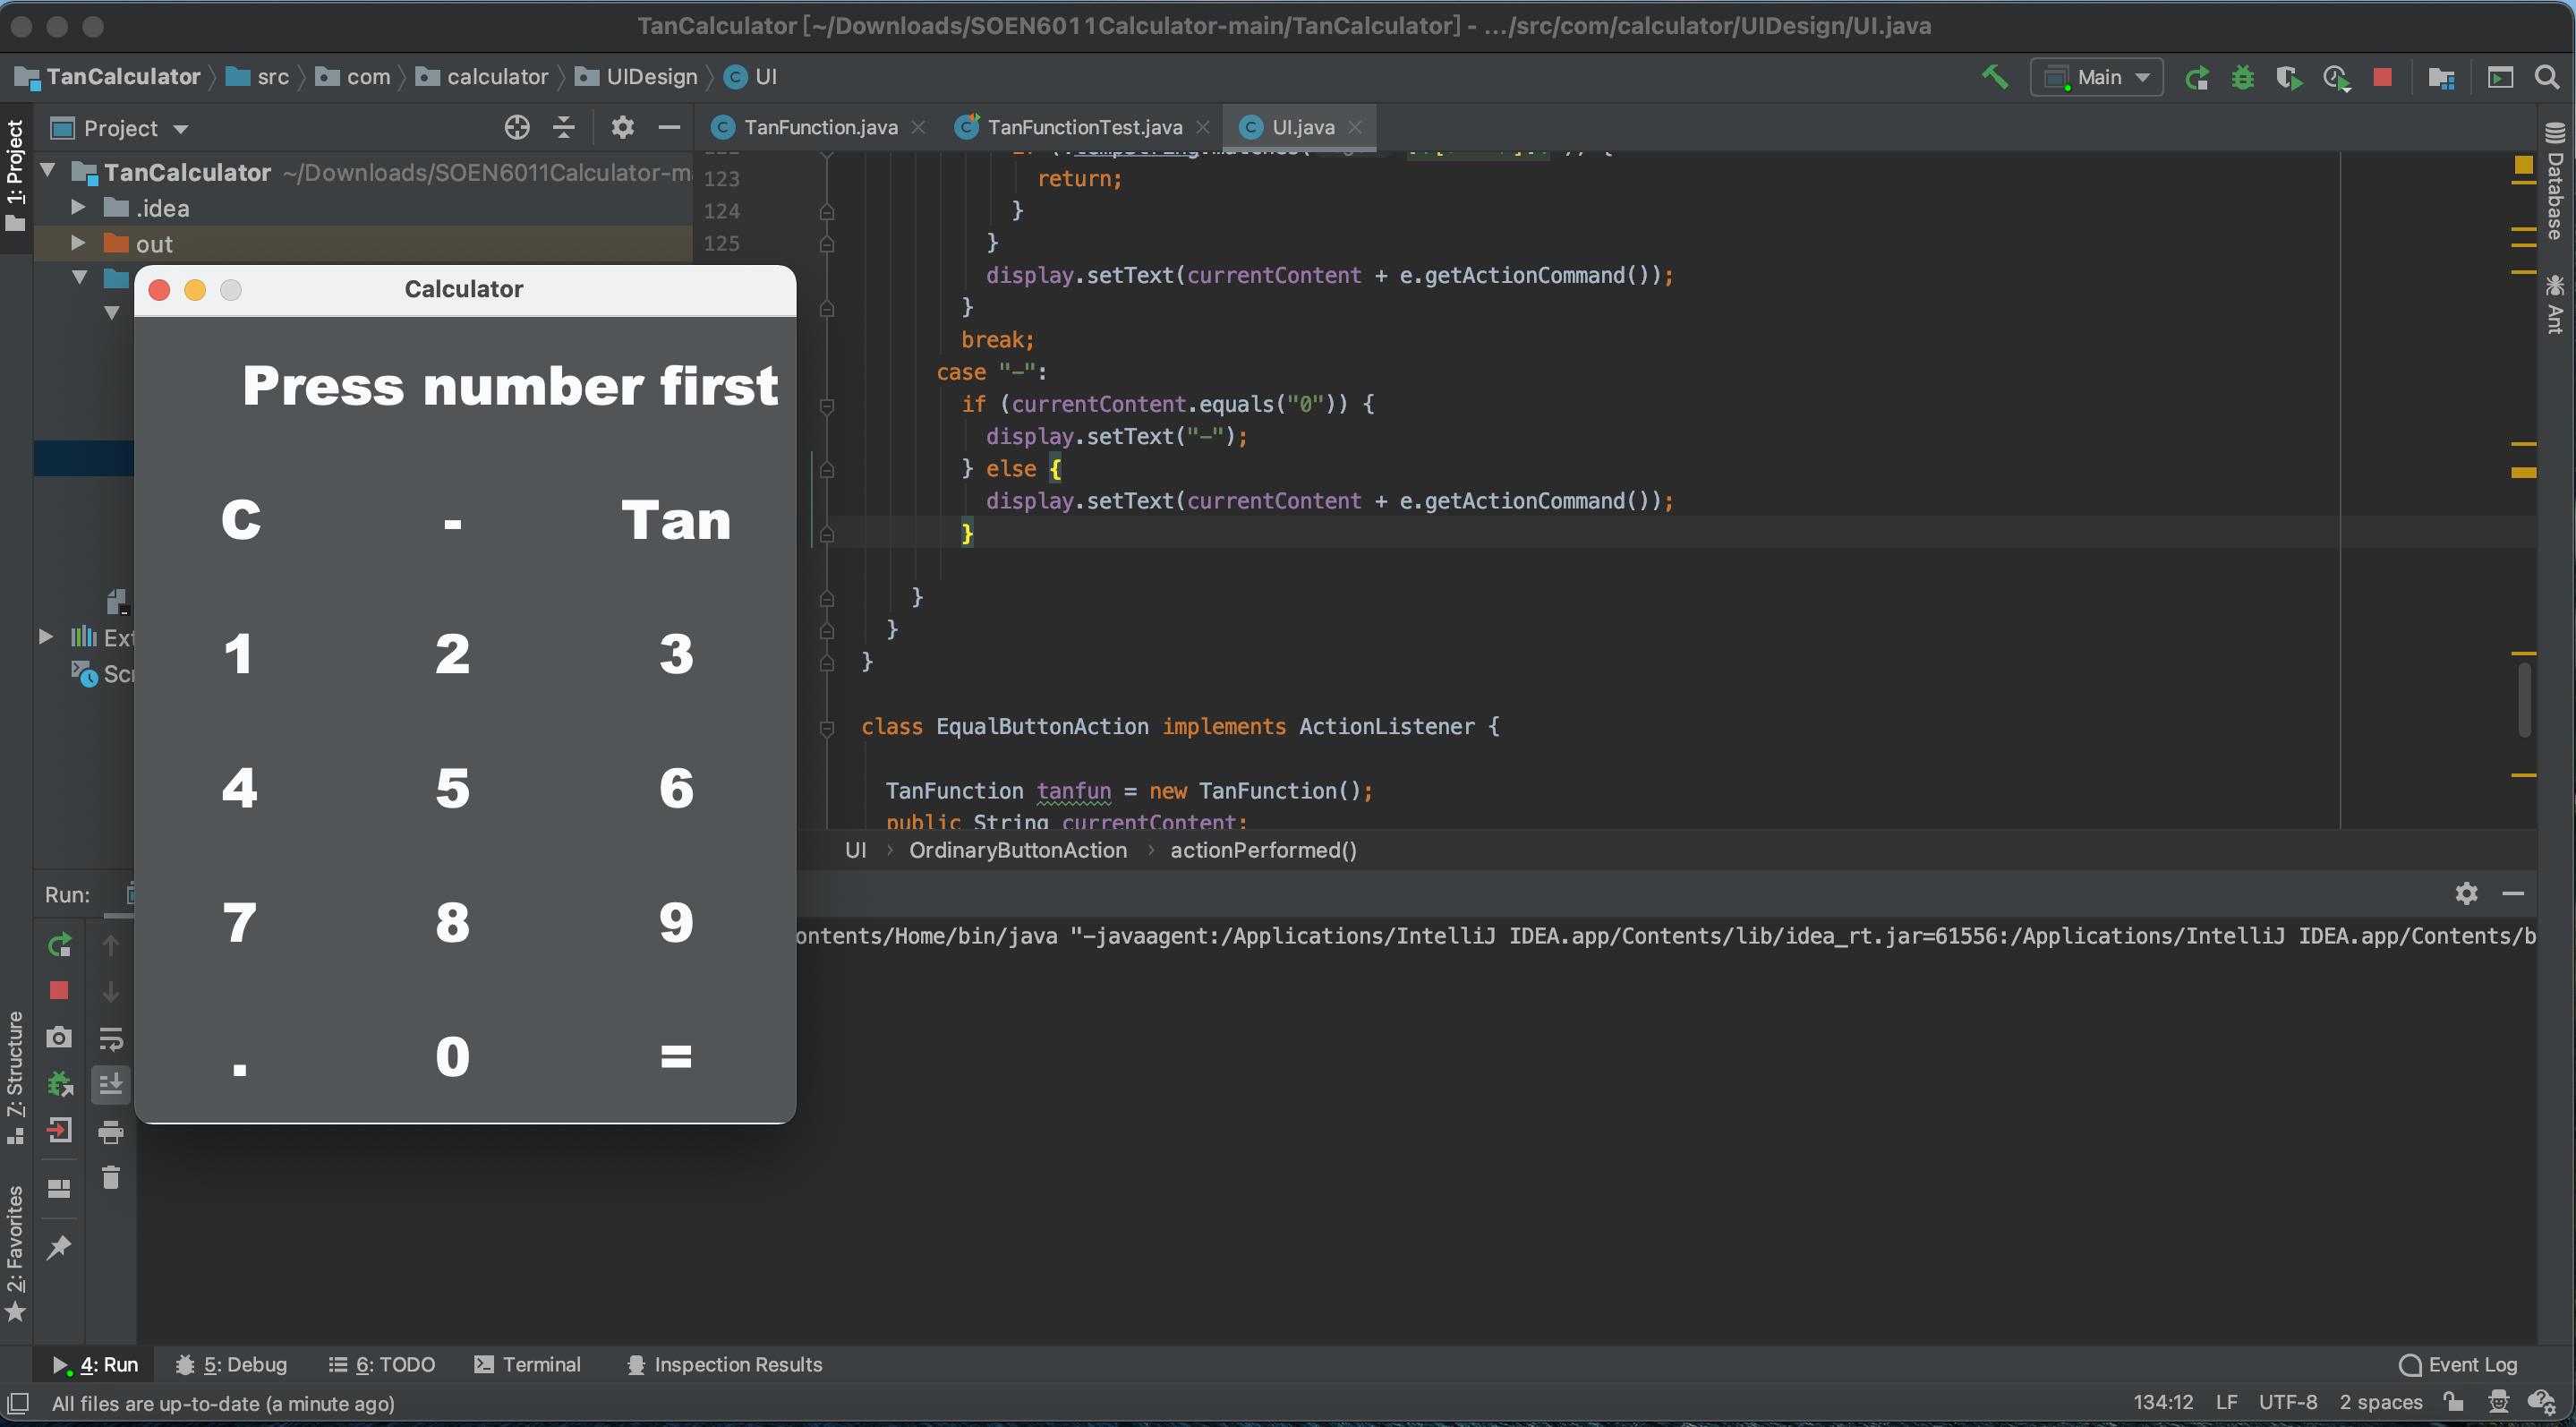
\includegraphics[width=13cm,height = 8cm]{err2}\\
\newline
This is the code to handle this error.\\
\newline
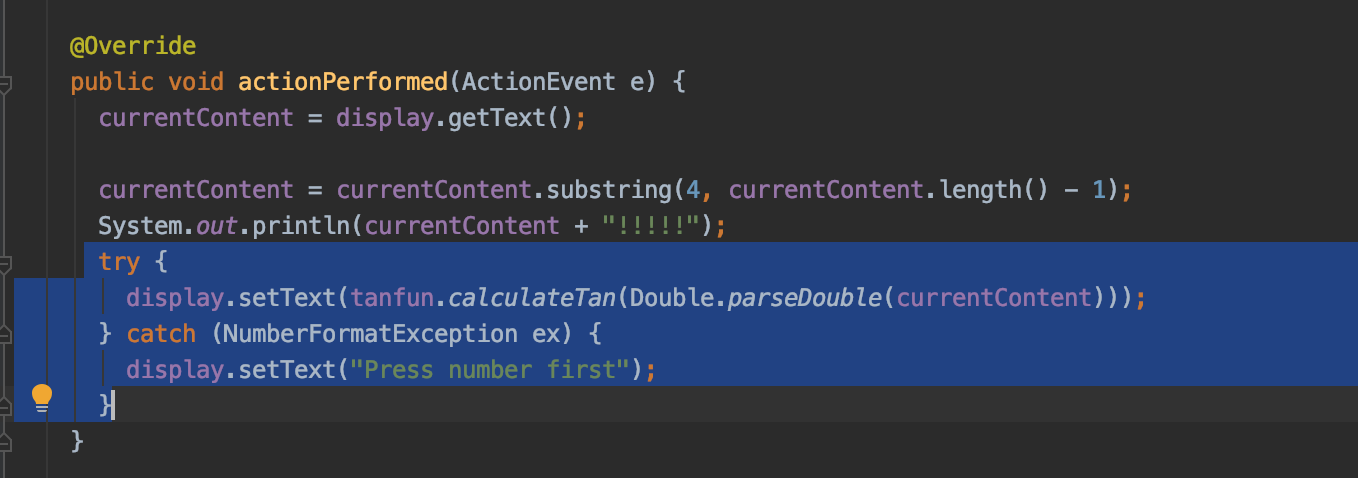
\includegraphics[width=13cm,height = 7cm]{err3}\\
\subsection*{c)Pragmatic Quality Checking Tool}\\
For code quality check part, I use Checkstyle to check the code quality.\cite{check}Checkstyle is a development tool to help programmers write Java code that adheres to a coding standard. It automates the process of checking Java code to spare humans of this boring (but important) task. This makes it ideal for projects that want to enforce a coding standard.\\
\newline
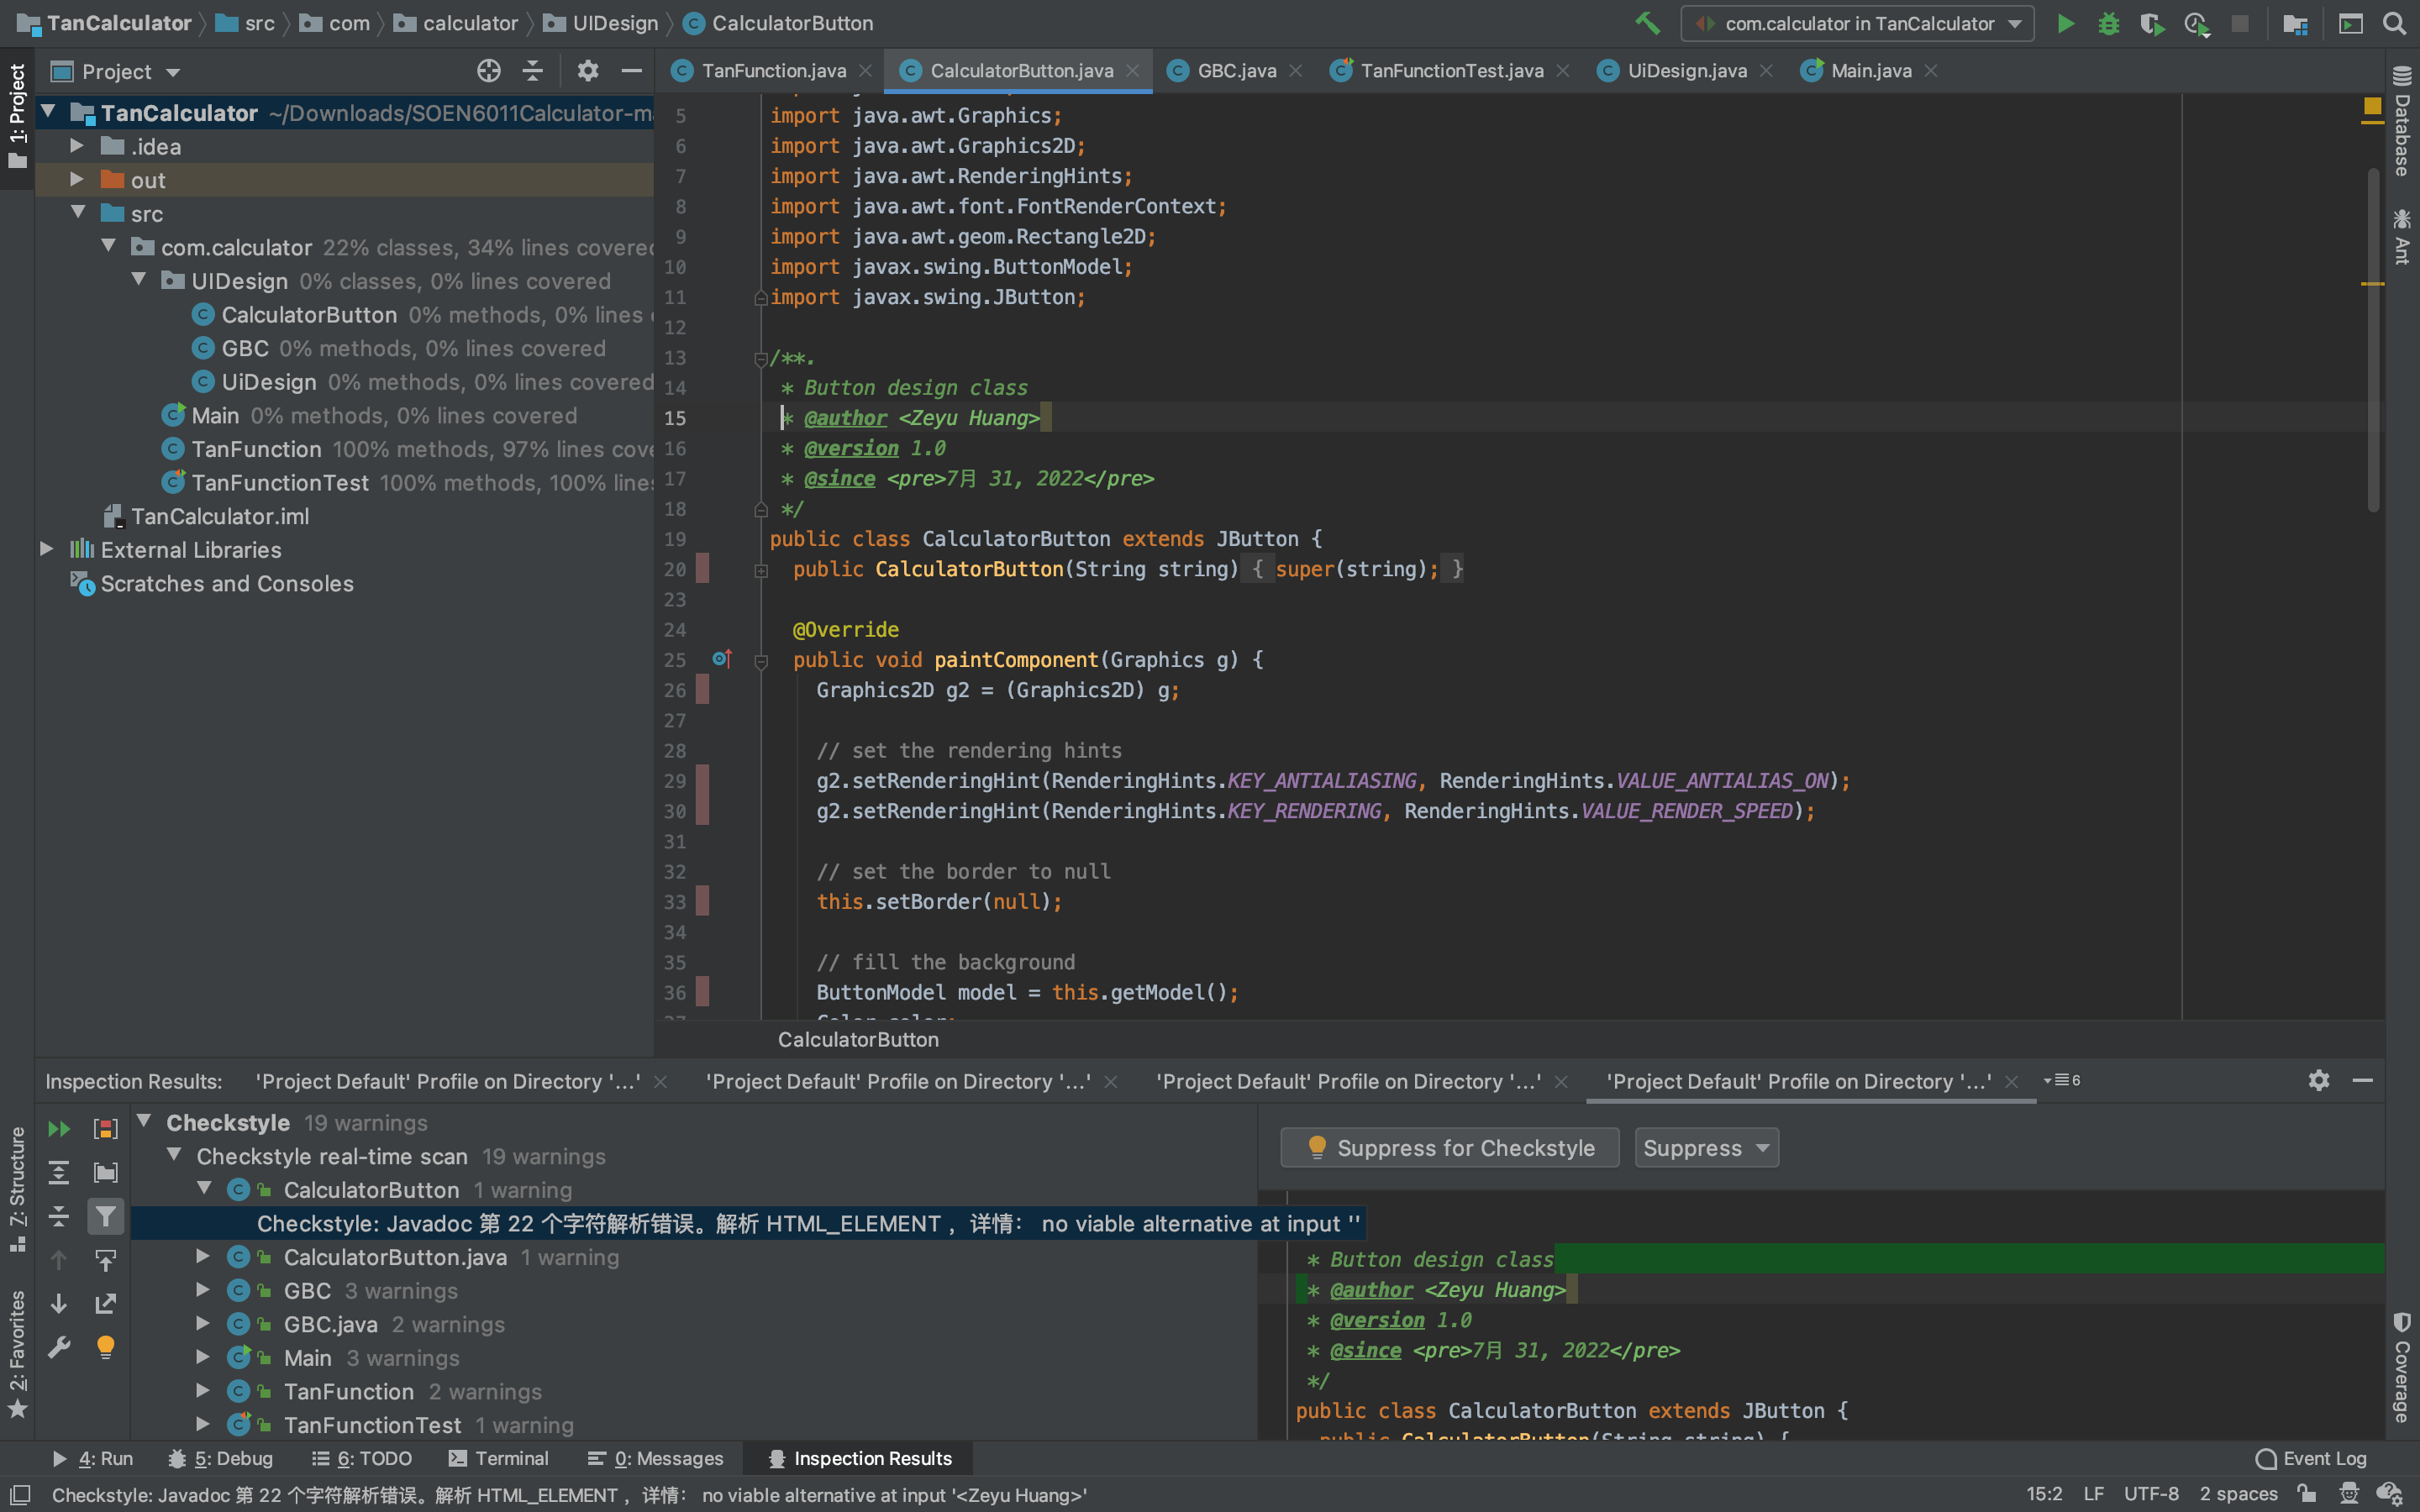
\includegraphics[width=13cm,height = 8cm]{check}\\
\newline
I use Checkstyle tool to fix some major warnings and errors, but left some unknown and unimportant warnings still not fixed.
\pagebreak
\newpage

\addcontentsline{toc}{section}{5) Problem 5}
\section*{5)Problem 5}\\
\textbf{Test Cases:}\\
\newline
\bigskip
\begin{tabular}{ |c|c|}
\hline
id & TC-01\\
\hline
Trace to requirement & FR1\\
\hline
Description
 & \makecell{To calculate the value of Tan(0)} \\
\hline
Precondition
 & The calculator is already on.\\
 \hline
Expected result
 & 0\\
 \hline
  Steps
 & \makecell{1.Enter 0\\ 2. Press "Tan" button \\ 
 3. Press "=" button \\ 4. Return 0 as output} \\
 \hline
\end{tabular} \\ \\

\newline
\bigskip
\begin{tabular}{ |c|c|}
\hline
id & TC-02\\
\hline
Trace to requirement & FR2\\
\hline
Description
 & \makecell{To calculate the value of Tan(195)} \\
\hline
Precondition
 & The calculator is already on.\\
 \hline
Expected result
 & 0.2679\\
 \hline
  Steps
 & \makecell{1.Enter 195\\ 2. Press "Tan" button \\ 
 3. Press "=" button \\ 4. Return 0.2679 as output} \\
 \hline
\end{tabular} \\ \\

\newline
\bigskip
\begin{tabular}{ |c|c|}
\hline
id & TC-03\\
\hline
Trace to requirement & FR3\\
\hline
Description
 & \makecell{To calculate the value of Tan(-10)} \\
\hline
Precondition
 & The calculator is already on.\\
 \hline
Expected result
 & -0.1763\\
 \hline
  Steps
 & \makecell{1.Enter -10\\ 2. Press "Tan" button \\ 
 3. Press "=" button \\ 4. Return -0.1763 as output} \\
 \hline
\end{tabular} \\ \\

\newline
\bigskip
\begin{tabular}{ |c|c|}
\hline
id & TC-04\\
\hline
Trace to requirement & FR4\\
\hline
Description
 & \makecell{To calculate the value of Tan(90)} \\
\hline
Precondition
 & The calculator is already on.\\
 \hline
Expected result
 & invalid\\
 \hline
  Steps
 & \makecell{1.Enter 90\\ 2. Press "Tan" button \\ 
 3. Press "=" button \\ 4. Return "invalid" as output} \\
 \hline
\end{tabular} \\ \\

\newline
\bigskip
\begin{tabular}{ |c|c|}
\hline
id & TC-05\\
\hline
Trace to requirement & FR1\\
\hline
Description
 & \makecell{To calculate the value of Tan(180)} \\
\hline
Precondition
 & The calculator is already on.\\
 \hline
Expected result
 & -0\\
 \hline
  Steps
 & \makecell{1.Enter 180\\ 2. Press "Tan" button \\ 
 3. Press "=" button \\ 4. Return -0 as output} \\
 \hline
\end{tabular} \\ \\

\newline
\bigskip
\begin{tabular}{ |c|c|}
\hline
id & TC-06\\
\hline
Trace to requirement & FR2\\
\hline
Description
 & \makecell{To calculate the value of Tan(45)} \\
\hline
Precondition
 & The calculator is already on.\\
 \hline
Expected result
 & 1\\
 \hline
  Steps
 & \makecell{1.Enter 45\\ 2. Press "Tan" button \\ 
 3. Press "=" button \\ 4. Return 1 as output} \\
 \hline
\end{tabular} \\ \\

\newline
\bigskip
\begin{tabular}{ |c|c|}
\hline
id & TC-07\\
\hline
Trace to requirement & FR2\\
\hline
Description
 & \makecell{To calculate the value of Tan(85)} \\
\hline
Precondition
 & The calculator is already on.\\
 \hline
Expected result
 & 11.4300\\
 \hline
  Steps
 & \makecell{1.Enter 85\\ 2. Press "Tan" button \\ 
 3. Press "=" button \\ 4. Return 11.430 as output} \\
 \hline
\end{tabular} \\ \\

\newline
\bigskip
\begin{tabular}{ |c|c|}
\hline
id & TC-08\\
\hline
Trace to requirement & FR2\\
\hline
Description
 & \makecell{To calculate the value of Tan(110)} \\
\hline
Precondition
 & The calculator is already on.\\
 \hline
Expected result
 & -2.7475\\
 \hline
  Steps
 & \makecell{1.Enter 110\\ 2. Press "Tan" button \\ 
 3. Press "=" button \\ 4. Return -2.7475 as output} \\
 \hline
\end{tabular} \\
\newline
\bigskip
For the test part, I use Junit testing framework to implement it. Below are the examples coverage and tests result.\\
\newline

\includegraphics[width=15cm]{images/Cover.png}\\
\newline
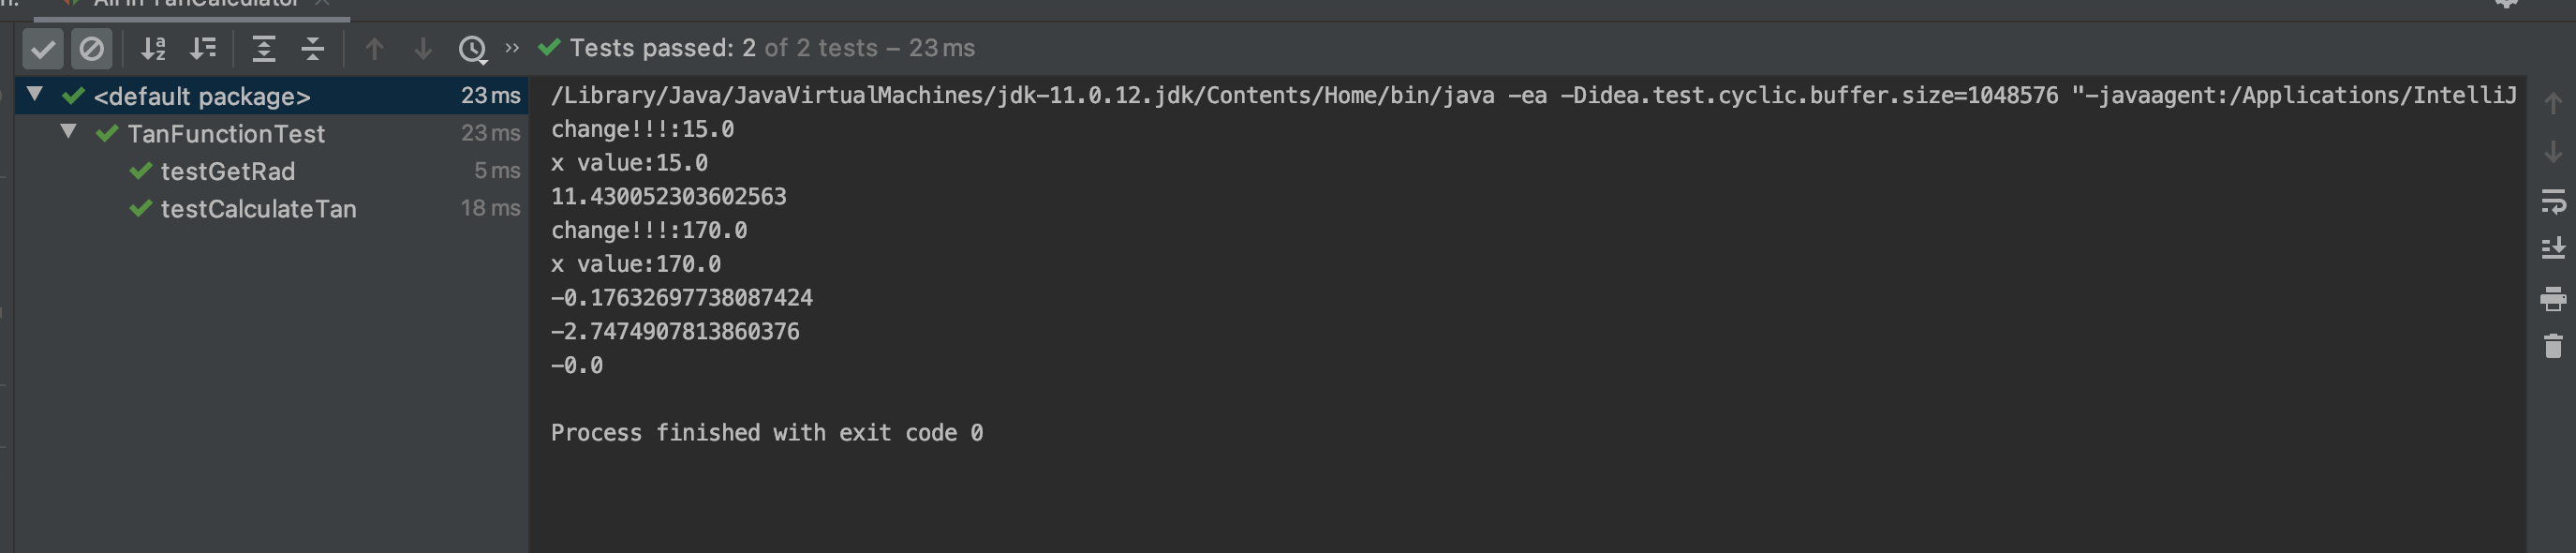
\includegraphics[width=15cm]{images/test.png}\\
\pagebreak
\newpage



\begin{thebibliography}{}
\bibitem{test1}
Varsity Tutors.
\\https://www.varsitytutors.com/hotmath/hotmath$\_$help/topics/tangent-function

\bibitem{varsitytutors} 
varsitytutors.graphing tangent function. 
\\https://www.varsitytutors.com/hotmath/hotmath$\_$help/topics/graphing-tangent-function

\bibitem{poly} 
Polynomial approximation
\\https://www.expii.com/t/what-is-a-polynomial-approximation-317
\bibitem{macl} 
Maclaurin series
\\https://mathworld.wolfram.com/MaclaurinSeries.html
\bibitem{pseupoly} 
Pseudocode for Polynomial approximation\\https://mathonweb.com/help\_ebook/html/algorithms.htm
\bibitem{check} 
Checkstyle\\
https://checkstyle.sourceforge.io/
\bibitem{Junit} 
Juit\\
https://en.wikipedia.org/wiki/JUnit
\end{thebibliography}
\end{document}
